\documentclass[12pt,UTF8]{ctexart}
\usepackage[utf8]{inputenc}
\usepackage{ctex}
\usepackage{geometry}
\usepackage{hyperref}
\usepackage{graphicx}
\usepackage{multicol}
\usepackage{multirow}
\usepackage{ulem}
\usepackage{longtable}
\usepackage{supertabular}
\usepackage{setspace}
\usepackage{keyindex}
\usepackage{enumerate}
\usepackage{url}
\def\UrlBreaks{\do\A\do\B\do\C\do\D\do\E\do\F\do\G\do\H\do\I\do\J
	\do\K\do\L\do\M\do\N\do\O\do\P\do\Q\do\R\do\S\do\T\do\U\do\V
	\do\W\do\X\do\Y\do\Z\do\[\do\\\do\]\do\^\do\_\do\`\do\a\do\b
	\do\c\do\d\do\e\do\f\do\g\do\h\do\i\do\j\do\k\do\l\do\m\do\n
	\do\o\do\p\do\q\do\r\do\s\do\t\do\u\do\v\do\w\do\x\do\y\do\z
	\do\.\do\@\do\\\do\/\do\!\do\_\do\|\do\;\do\>\do\]\do\)\do\,
	\do\?\do\'\do+\do\=\do\#}


\geometry{left=3.0cm,right=3.0cm,top=3.0cm,bottom=3.0cm}
\title{
	\textbf{\fontsize{18.2}{1} 时代的一粒沙,落在每一个人头上,都是沉重的一座山}\\
	\large{—— “中考分流”背景下中学生教育评价体系的研究与对策}
}
\author{初三二班\\叶致诚\quad 朱汶宣\quad 张育维\quad 戚若渝}

\begin {document}

\begin{titlepage}
	\newcommand{\HRule}{\rule{\linewidth}{0.5mm}}
	%\includegraphics[width=8cm]{title/logo.png}\\[1cm] 
	\center 
	\quad\\[1.5cm]
	\textsl{\Large Shanghai Foreign Language School Affiliated to SISU }\\[0.5cm] 
	\textsl{\large 上海外国语大学附属外国语学校}\\[0.5cm] 
	\makeatletter
	\HRule \\[0.45cm]
	{ \huge \bfseries \@title}\\[0.45cm] 
	\HRule \\[1.5cm]
	\begin{minipage}{0.45\textwidth}
		\begin{flushleft} \large
			\emph{作者:}\\
			叶致诚\ 朱汶宣\ 张育维\ 戚若渝
		\end{flushleft}
	\end{minipage}
	~
	\begin{minipage}{0.45\textwidth}
		\begin{flushright} \large
			\emph{指导老师:} \\
			\textup{董涛玲}
		\end{flushright}
	\end{minipage}\\[3cm]
	\makeatother
	{\large 上外附中初三社会实践}\\[0.5cm]
	{\large 初三二班}\\[0.5cm]
	{\large \today}\\[2cm] 
	\vfill 
\end{titlepage}

\maketitle
\begin{abstract}
	
	在目睹了当前职业教育法以及新课标下五五中考分流的诸多争议之后,我们发现了新时代对技术工人提出的新要求,以及中考分流所带来的心理压力和知识结构的不完整;发现社会实践在中小学十分流于形式,青少年普遍缺乏创新精神。我们决心研究中小学评价机制的改进方案。我们通过问卷调查,文献分析以及对学生、家长、老师进行访谈,从而对当下情况有了较为全面的了解。针对当前问题,我们提出了将中考的分流属性延缓到高中一年级再实行的办法,与此同时改革中学课标以达到教学内容连贯化,教学方式区分化的效果;我们提出如鼓励民间资源和公有力量充分结合的建议改善当前中小学社会实践,使社会实践质量更高,普及范围更广。我们提出如调整评价模式激励学生动力的建议发展学生的创新能力,使创新精神不再成为空谈,而是成为中小学生的必要的能力。
\end{abstract}
{\centering {\textbf {关键词}}\\
	\centerline{教育;中学教育;职业教育;中考分流;创新能力;素质教育;社会实践}}
\newpage
\tableofcontents
\newpage

\section {绪论——从中考分流政策说起}
\subsection {概念界定}
\paragraph {中考与普职分流}
初级中等教育毕业考试,简称“中考”,是中国大陆地区对于初中毕业生所设置的全国性考试。\footnote{\url{https://mp.weixin.qq.com/s/WHYkcF5M6mKKuEwBP_esdQ}}
普职分流指于 1985
年中央深化教育体制改革以来普通高中与中等职业学校在生源上的分流。我们社会实践的讨论重点,即“五五分流”,为我国高中阶段教育坚持普通高中与中职学校招生比例大体相当的政策\footnote{《民进中央:关于尽快调整完善高中阶段“普职分流政策”的提案》
	\url{http://cpc.people.com.cn/n1/2022/0228/c442045-32361825.html}}。 
根据教育部于 2021 年 10 月发行的《关于推动现代职业教育高质量发展的意见》\footnote{奔流新闻《教育部明确!坚持普职分流、支持试办职业本科》
	\url{https://www.thepaper.cn/newsDetail_forward_16823776}},当前,中职教育主要存在办学定位不适配,办学规模大而不强,办学条件缺口大等问题。但仍要坚持普职分流、支持试办职业本科。

\paragraph {初中学生综合素质评价}
初中阶段的综合素质评价是上海市初中生需要面对的一项考核。以上海市的初中学生综合素质评价信息管理系统为例,该平台记录一名初中学生自六年级以来在品德发展与公民素质,休息课程与学业成绩,身心健康与艺术素养,以及创新精神与实践能力四个方面的成就和能力。
包括但不限于社会考察,公益劳动,职业体验,安全实训,探究性学习等项目。
根据《上海市初中学生综合素质评价实施办法》\footnote{上海市教育委员会关于印发《上海市初中学生综合素质评价实施办法》的通知
	\url{http://edu.sh.gov.cn/zcjd_area_3679/20200706/0015-xw_99991.html}},初中学生的综合素质评价有以下四个版块:
\begin {itemize}
\item [1)]
\textbf{品德发展与公民素养。}主要反映学生践行社会主义核心价值观、弘扬中华优秀传统文化等方面的表现,包括爱党爱国、理想信念、社会责任、集体意识、诚实守信、仁爱友善、遵纪守法、安全素养、文明礼仪等。重点记录学生遵守日常行为规范方面的表现,参加社会考察、公益劳动、职业体验、安全实训、共青团和少先队等德育活动、国防民防教育活动的情况。
\item [2)]
\textbf{修习课程与学业成绩。}主要反映学生初中阶段各门课程知识和技能掌握情况以及运用知识解决问题的能力等。重点记录基础型课程成绩、拓展型课程和探究型课程的学习经历。
\item [3)]
\textbf{身心健康与艺术素养。}主要反映学生的健康生活方式、卫生保健、体育锻炼习惯、身体机能、运动技能和心理素质,对艺术的审美感受、理解、鉴赏和表现的能力。重点记录《国家学生体质健康标准》测试结果,参加体育运动、健康教育、艺术活动经历及表现水平等情况。
\item [4)]
\textbf{创新精神与实践能力。}主要反映学生的创新思维、调查研究能力、动手操作能力和实践体验经历等。重点记录学生参加探究学习、科技活动等方面的过程和成果。
\end {itemize}

\subsection {研究背景}

\par{四月的中国互联网上,关于新版《中华人民共和国职业教育法》(简称“教职法”)的讨论屡屡登上了热搜,网民们再次激起了对于“中考是否决定命运”的讨论。\footnote{中华人民共和国职业教育法
		http://www.npc.gov.cn/npc/c30834/202204/04266548708f44afb467500e809aa9cf.shtml}无论是四月初时一片普天同庆的场面,亦或是四月末官方的一片片辟谣浇灭了大家的那一份惊讶。\footnote{澎湃新闻《【网络辟谣】普职分流“取消”了?教育部回应》
		\url{https://m.thepaper.cn/baijiahao_17871440}}
	不难发现,中考分流政策在社会上存在重大争议且是大多数人都在密切关注的问题。}

\par{教育部关于做好 2020 年中等职业学校招生工作的通知\footnote{教育部办公厅关于做好2020年中等职业学校招生工作的通知
		\url{http://www.moe.gov.cn/srcsite/A07/moe_950/202005/t20200511_452724.html}},第一条就明确要求坚持职普比例大体相当,适度扩大中职招生规模,同时要求加强宣传引导力度。明显可以看出,在短时间内有限的社会资源不可能让所有人都走进高等教育的殿堂。与之相对的,中等职业学校的就业不成问题,其就业率高达
	95\% \footnote{《中职生就业率超 95\% 高就业率难掩中职教育之窘》
		\url{https://zyzd.org/jiaoyudongtai/3273.html}},数据上大于本科生的比率。}

\par{但是从中职网的评论文章中可见,中等职业学校的毕业生们所从事的职业只是基础的体力劳动,而无法达到中职所能培养出来的技术型人才的要求。根据德国Statista公司的报告显示\footnote{\url{https://www.statista.com/statistics/252912/monthly-salary-of-university-graduates-in-china/}},2020
	年大学生的平均毕业薪资为 5471 元,相比之下高职生的薪资只有 4253 元,而根据澎湃新闻 2021
	年的报道显示\footnote{澎湃新闻《被指差生代名词,就业起薪近七成不足三千,中职生出路何在》
		\url{https://m.thepaper.cn/baijiahao_15583458}},近七成的中职毕业生的工资不到 3000
	元。单从金钱的差距就可以体现出高等教育对于一个学生未来的重要性。}

\par{这就不是凭借努力就可以改变的事情了。中国发展研究基金会对广东、四川、贵州三省 30 所中等职业学校的跟踪研究发现, 在这些学校,70\%
	的生源都来自于农村\footnote{《中国发展研究基金会发布报告:中等职业教育应注重质量提升》
		\url{https://gdjy.axhu.edu.cn/contents/2847/142427.html}}。城乡之间的巨大差距会进一步的导致阶级流动机会的丧失,在低端劳动力需求低下的今天,无疑分流会导致他们陷入循环,难以得到出头之日。}

\par{坐在魔都的大厦楼宇间的我们可能很难体会到这样一场残酷而盛大的决斗会给在山区县城的千万学子带来什么样的结果。这可能是新的希望,也可能是灰暗的绝望。我们希望去用自己的足迹寻觅这个答案。尽管疫情阻拦了我们在市井间行走的脚步,但是通过线上的访谈和邻里间的交流——我们希望通过一个个鲜活的故事,去探求到在同一片天空下人与人之间的岔路会引向怎样不同的结局;希望通过一点点思想的火花,让我们从中小学生、高中生,大学生,亦或是教育从业者的角度看待当代的中国教育环境。}

\par{在目睹了中考分流的诸多争议之后,我们将目光投向当前的体制中。根据教育部最新的制定的义务教育课程方案(2022
	年版)\footnote{\url{https://hudong.moe.gov.cn/srcsite/A26/s8001/202204/W020220420582343217634.pdf}},以体育和艺术为代表的素质教育类课程的占比在逐步提升,两者在总课时中的占比之和可以与语文的课时量相媲美,遥遥领先于外语和科学探究课程。这项改变表明了我国逐步计划迈向更加全面的教育阶段。可惜的是,目前社会上还没有多少案例能证明目前的改变为我国素质教育事业带来实质的变化。另一方面,当前课标中对于不同学科难易程度仍然有很多可以斟酌的地方,例如语文的古诗文占比和写作难度,数理化的深度和广度,外语课程的开展形式等。这些大大小小的困难和纠结不仅会因地域和城乡发展不均匀造成的师资差距带来负面影响,同样会持续影响着那些初高衔接的学生。}

\par{与此同时,上海市中学生综合素质评价信息统计系统在上海面世,一时轰动教育界。正如斯塔费尔比姆曾指出:“评价最重要的意图,不是为了证明而是为了改进”,这类网站应作为教育信息电子化的标志伴随着学生的生涯,以忠实的记录者和监督者身份为中小学建立完整的“成长档案”,同时也为学生在社会上开展职业体验和自主探究保驾护航。因此,我们想试问:这些理念和平台是否能成为这个应试教育穹庐下的突破口呢?}

\subsection {研究意义}
\par{在互联网上中考分流的议题拥有很高的讨论度。经过我们的观察,主流媒体和社会舆论主要聚焦考生们该如何应对新政策,同时注重分析这样的政策会释放怎么样的信号。根据中国知网的检索结果,多数的研究文章还仅仅是拘泥于政策相关时事和职业教育发展前景这两大话题。举例说明:在知网上检索“中考分流”字样,只有一篇硕士论文和一篇学术期刊。主题也是关于中考分流和进城务工人员之间的关系。“普职分流”则干脆没有任何学术论文加以研究,可见当前教育界对中考分流问题研究的匮乏。}

\par{基于上述事实,我们得出结论:对于“如何改善/调整中考分流政策”这一话题,社会上发声的媒体和群体还是少数。我们希望能够提出有创意的、行之有效的解决方案,让更多的人听到不一样的声音,从而改善社会中小学教育系统。}

\par{与之不同的是,通过查找和寻证,可以了解到近年来多地对于各阶段的综合素质评价体系都有较多的研究分析,例如黑龙江大学的吕欢发表于黑龙江科技的《义务教育中综合素质评价实施存在的问题及对策研究》\footnote{吕欢,黑龙江大学《义务教育中综合素质评价实施存在的问题及对策研究》
		\url{https://kns.cnki.net/kcms/detail/detail.aspx?dbcode=CJFD&dbname=CJFDLAST2022&filename=HELJ202203005&uniplatform=NZKPT&v=jq1xnrYj1PzMhzcC_LWKxs2wkrD8KkAOr--x9sDpFOZcMU3KL3grHKzmP4GtXrIt}}就进行了宏观层面的分析。}我们希望以学生的身份,通过了解不同省市不同层面的同学和老师在教学中的亲身感受去探求对于目前的评价系统存在怎么样具体的问题,同时结合各地学校的优秀案例提出现实的解决方案,帮助素质教育落到实处,发挥应有的效果。
\newpage

\section {调查方法}
\subsection {文献分析法}
\par{在我们开始研究之前,我们首先对有关中考的政策文件进行了研究,主要包括新制定的《职业教育法》、中小学新课标以及近几年来中央教育部和全国各地教育部门对于中考分流的基本政策和具体执行情况。这为我们了解决策者制定改写政策的理想目标及心理活动有很大帮助,也为我们之后进一步的研究指明了方向。}

\par{在社会实践的具体操作上,我们运用互联网工具和“中国知网”等相关平台查寻资料辅助探究,充分了解社会各方面对于分流政策的态度。在阅读分析和思考讨论的基础上获得启发。发现当前评价机制中可能存在的问题,从而得出更有效的结论。}

\par{在得出研究结论的过程中,我们也参考了一些全国政协委员和人大代表们提出的建议进行了思考与研究,并从中汲取精华部分加入到我们的研究中来,辅助我们得到最后的解决方案。}

\subsection {问卷调查法}
\par{本次社会实践我们采用了问卷星这一线上问卷制作平台,多种问卷散步途经,如微信朋友圈,知乎,QQ,百度贴吧,微信公众号,邀请家人朋友二次传播等发放问卷,收集数据。经过
	5 月 1 日至 5 月 5 日共计 5 天的收集,共收集到了 797 份问卷,其中,作答时间过短或者问答题内容不符合要求的无效问卷共 63 份,有效问卷一共
	734 份。}

\par{我们从我们的研究主题出发,针对社会面对于现阶段中考分流政策的看法;对于初中学生综合素质评价系统的态度;对于中学生创新实践能力的评价三个维度做出调查。这其中,我们的调查覆盖了小学至
	55 岁以上成年人的各个年龄段,囊括了当今社会的各种职业进行调查。回答问卷的人群中,包含未成年人 186 人(25.3\%),成年人 548
	人(74.7\%);在所有答卷的成年人中,有 390 人(71.2\%) 表示自己是家长,有 66 人(12.0\%) 表示自己是老师;在成年人中,占比最高的是
	41 至 55 岁的人,有 266 人,占了成年人总人数的 48.5\%;26 到 40 岁的人也有不少,有 193 位,占成年人总人数的 35.2\%。}

\par{
	在收到的问卷中,有部分填写者在既定区域给予了我们宝贵的建议,提出了自己对于当前现状和改进方案的想法,其中的部分具有一定参考价值,有助于思路的拓宽和思考建议的充实。}

\subsection{案例访谈法}
\par{为了更为细致地了解不同社会层面的人士对于中小学评价体系的看法,我们向来自上海市区,崇明区,南京市,北京市等全国不同地区的人群
	开展了针对性的访谈。访谈覆盖的人群丰富多样,主要囊括了各个学科的教育工作者、不同年龄段和教育模式的在校学生和家长。覆盖了体制内和体制外、中考生和保送生等多种人群,尽可能保证了样本的覆盖性和广泛性。}

\par{访谈形式在市区受到疫情条件限制,主要局限于腾讯会议访谈和文字沟通;在崇明区以线下访谈为主。根据受访者的身份和学校/毕业院校的信息,询问了他们关于当前中考政策的看法以及身边人在中考前后的经历故事。迥异的背景让我们认识到了不同成长路径会使学生对于中考分流以及综合素质评价体系有截然不同的认识,也为之后讨论对策方案提供了思路方向和启发。}

\newpage

\section {实践过程}
\subsection {中考分流所带来的弊端和时代所需要提出的要求}
\subsubsection {对于高中课程的适应性}
\par{在体制内就读普通高中的同学皆表示,初中与高中的课程在教学和设计方面都有较大的不同。教授课程的时候,高中老师对于学生的自学能力有更高的要求,不会像初中老师一样无微不至地告诉学生需要重点记录的知识点,同时紧盯学生的进度,时刻关注学生的学习状态。这点是造成了学生在初高中阶段学习成绩波动较大的主要原因。而课标的不妥当导致了这个现象。}

\par{同时在访谈中,我们了解到,学生们普遍认为化学和生命科学两门课程在无法接轨的问题上尤其严重。以这两科为例,我们在互联网上检索了义务教育化学课程标准(2022版)和义务教育生物学课程标准(2022版)\footnote{中华人民共和国教育部http://www.gov.cn/zhengce/zhengceku/2022-04/21/5686535/files/87e97b349df8484bb003a41419b97839.pdf/中华人民共和国教育部
		\url{http://www.gov.cn/zhengce/zhengceku/2022-04/21/5686535/files/04b3a45e2504464bb61a2a3590a8e860.pdf}},其中目标要求部分就写明了需要掌握的主要是两门科学中的基础知识以及培养生命/化学观念,初步发展相应思维能力,以及科学实践能力,尤其是实践方面,有大量必做实验,还有总占比达10\%的跨学科项目。}

\par{然而,当我们翻阅例如普通高中化学课程标准(2017版)\footnote{中华人民共和国教育部
		\url{http://www.jwc.ecnu.edu.cn/_upload/article/files/f7/28/dc6ae6dc46faa43b343da2b24d7a/70bc6036-a93c-40e8-a4e3-af165ea53534.pdf}},发现其必修部分在涉及方面上和义务教育阶段有相当部分的重合,例如《义务教育课标》中的2.2.3和《普通高中课标》中的2.4同样是谈论金属的性质,且要求上没有显著区别;《义务教育课标》中的第三部分“物质的组成与结构”和《普通高中课标》中的主题三“物质结构基础与化学反应规律”中,都涉及到了原子结构和物质组成等内容,存在重叠现象。}

\par{因此可以理解为,初中部分的化学学科只做了学术上的引入,不提供具体的解释,而留在高中再做深入讲解。但与此同时,上海市的学校大多在九年级开展化学课程,这样的大纲部分重合容易导致学生的概念混淆和知识点的相互矛盾,反而不利于学生的继续学习。}

\par{和我们的想法一样,受访者普遍表示理科学科初中阶段知识体系不完整,教的浅。对于其中反响最严重的化学学科,比较典型的是我校初二黄同学的案例,她向我们表示:
	\begin{quote}
		\kaishu 初中化学太散了,没有建立知识体系。解决办法是把内容放紧凑一点,或者多教一年化学。
	\end{quote}
	存志中学的王同学对数理化课程的安排也提出了自己的见解:
	\begin{quote}
		\kaishu
		化学课标所有人都觉得不完整,零零散散的,应该多教一点;数学也不完整,初高衔接有脱节。难度有跳跃,不容易跟上;物理进行了拓展,提前讲了高中的知识。
	\end{quote}
	当然,这种结论也是因人与校而异的。我们同样收集了一些关于英语和其他学科的意见。一位来自浙江的前清华学长,现 MIT 学生金同学表示说:
	\begin{quote}
		\kaishu 我记得我们初中教的英语比较难,经常给我们补充高中难度的内容,然后到了高中就感觉英语课有点水, 这个感觉效率不够高;理科的话,
		感觉初中几乎啥都没教, 然后高中又教的比较快。
	\end{quote}
	对于数学教学,我们采访了陆云舟老师,他指出高中不适应在当前教育体制下是必然,因为高中学科的学习对于学生的综合要求较高:
	\begin{quote}
		\kaishu
		从数学学科上来说,数学在初中阶段主要需要同学们有一定计算能力和简单的几何推理能力。高中数学对同学们的逻辑思维能力要求更高,尤其是抽象思维。两个学段侧重点不同必然会出现初入高中后不适应的同学。
	\end{quote}
	我校化学教师李启翔同样点出了初高中学习模式的不同:
	\begin{quote}
		\kaishu
		初中和高中学习的要求是不一致的,初中可以依靠突击、记忆解决,而高中学习的要求决定了要面对更重的压力,需要及时更新学习进度和要求,这一点来说初中简单的临阵磨枪的方法已经完全无效了。
	\end{quote}
	一位拥有30余年教龄的,曾经教过初中与高中的英语张老师表示:
	\begin{quote}
		\kaishu
		高中英语不管是在阅读面,词汇量方面,对于文本的理解都一种深层次的考研,而初中的很大一部分老师都不是很看中英语听说读写当中的读和写,所以随着难度深度广度的增加,有很多学生对于高中的学习是十分不适应的,体现出一种初中高分低能的表现,他们并没有为高中学习做好准备。
	\end{quote}
	
	从中我们不难发现,适应高中的学习需要学生一定的逻辑思维能力以及很好的学习方法。这便导致了很多同学在进入高中之后不适应,能力不够,无法顺利继续学业的现象。这种现象呼唤社会改进当前课程标准以来解决这种问题,我们稍后会详细进行探讨。
}
\par{
	而初高衔接中出现的问题,其中有很大一部分和老师的教学手段和教学方法挂钩。这一点从南京外国语学校的Z同学的肺腑之言中可见一斑:
	\begin{quote}
		\kaishu
		初中课程上的质量如何与老师关系比较大。我的切身体会就是感觉初中有一些毫无意义的抄写作业,还有理科(特别是数学)做了太多无意义的简单题,导致考试的时候一些稍微难一点的题很多同学(包括我)会停顿甚至做不出来。换句话说,感觉初中文化课对思维提高的锻炼和引导还不够。
	\end{quote}
	从老师的角度出发,英语张老师也表示:
	\begin{quote}
		\kaishu 现在初中到高中的课程的衔接不是很合理,具体来讲初中英语有很多内容是能通过机械性的操练得到提升的。
	\end{quote}
	初中课程体系不完整,也是初高衔接有苦难的罪魁祸首。我校高一的一位学长没有机会体验到学校教导处精心安排的衔接改革课程,只能接原版教学,所以曾吐槽道:
	\begin{quote}
		\kaishu
		像是数理化感觉初中确实讲的不完整,像是数学把集合放到高中,反证法不能用之类的,然后化学初中好像什么都没学,到高中把初中的东西基本上推翻重来,包括物理也是的。感觉到高中以后初中很多东西就是错的,是非常无聊的。
	\end{quote}
	此可见,初中教学课程不完整,不仅仅会影响学生的心态和状态,甚至还会错失锻炼引导批判性思维的机会,树立错误的知识点印象,并且还会影响学生对学科的探究积极性。
}
\par {
	
	受访者普遍认为,尤其对于科学类课程,高中的难度较初中有显著提升,而更加雪上加霜的是,学生们一致同意初高中课程缺少接壤,两者的断层也使学生难以直接适应新的节奏。正是因为如此,体制内的很多同学普遍表示,初高衔接有着相当的困难。来自苏州某私立高中的尤同学表示:\begin{quote}
		\kaishu 到高中前也没有足够的心理准备,自己也因为不喜欢高中老师的态度导致没有认真学习,在高一阶段缺乏调整的前提下逐渐落入从优等生落入中流。
	\end{quote}
	同样就读于体制内学校的,在保送考中不幸落榜导致参加中考的——来自标化直通车机构,拥有17年托福雅思SAT培训教龄的叶叶老师向我们表示:
	\begin{quote}
		\kaishu
		开学第一次数学月考全班只有两个人及格了,一个60一个62。自己没及格,感觉人生跌到了谷底,就是在高中之前,不及格的感觉就像是天塌下来一样的,所有家长被约谈。衔接和课程都很有难度。
	\end{quote}
	相比下,初高中一体化的学校(例如上外附中,星河湾一类的国际学校等),学生大多较少反映这种类型的问题,体现出初高衔接的重要性和必要性。
}
\par {
	从老师的角度出发,我校英语教师陈老师在访谈中表示:
	\begin{quote}
		\kaishu
		我们学校课程安排的难度更像是逐步的上升,不会给学生带来太多的额外压力,并且固定的环境也有助于保持学习状态。所以心理波动较大的同学大多是因为家长的压力和预期或者是青春期的问题,而不是因为学业上的问题。
	\end{quote}
	我们研究的另一个典型案例上海耀中外籍人员子女学校,一所十三年一贯制,从小学到高中建立完整知识体系的国际学校。就读于这所学校陈同学在访谈中表示:
	\begin{quote}
		\kaishu
		因为我们学校本来就是一贯制学校嘛,所以课程是很连贯的,初高谈不上困难。难度差距还是有一点的,高中考试最开始没有初三发挥稳定,但一会儿就适应了。
	\end{quote}
}

\subsubsection {中考压力太大,一考定终身}
\par {在大部分人的认知当中,因为各种因素,中考会给学生巨大的压力。这点在诸多社会调查中得以体现。伦敦大学学院的 Therese Hesketh 教授在一份
	2013 的报告中就表示,每三个中国中小学生中就有一个学生因为应试教育系统而承受心理上的压力。\footnote{Dong Fangyu, 2013,
		\url{http://global.chinadaily.com.cn/a/201308/23/WS5a2f8f14a3108bc8c6726ee9.html}}
	而在新冠疫情肆虐的今天,Li
	等在2020年发布的数据显示,中国学生的总体抑郁症罹患率在疫情前后并没有太大的变化,分别是22\%和22.2\%。\footnote{Li JY, Li J,
		Liang JH, Qian S, Jia RX, Wang YQ, et al. Depressive symptoms among children and
		adolescents in China: a systematic review and meta-analysis. Med Sci Monit Int
		Med J Exp Clin Res. (2019) 25:7459–70. doi:
		10.12659/MSM.916774}。这样居高不下的状态说明了是疫情之外的因素导致了学生的焦虑,而背后的原因大概率就是考试压力。同时,Chi 
	等在2020年开展的研究说明,学习成绩差是导致学生患有严重抑郁的直接因素之一。\footnote{Xinli Chi,XiaofengLiua,Qiaomin
		Huang,LiuyueHuang,Peichao Zhang,Xiaochen Chen,2020年9月, Depressive Symptoms Among
		Junior High School Students in Southern China: Prevalance, Changes, and
		Psychosocial Correlates,
		\url{https://www.sciencedirect.com/science/article/abs/pii/S016503271932779X}}在中考中分流和竞争的压力也不言而喻了。}
\par{
	
	本次的受访者有很大一部分用各种办法避开了中考的激烈竞争,有些受访者可以参加校内直升,也有的直接与学校签约,因此多数表示他们在参加考试时都没有太过显著的紧张情绪。我们的主要研究对象是传统的体制内中考,所以首先对这一群体进行研究。我们发现,在体制内学校,中考所带来的压力很大程度上和一个人平时的学习表现挂钩。即将面临中考的存志中学初三王同学和我们分享了他的心态:
	\begin{quote}
		\kaishu 张弛有度,不紧不慢。
	\end{quote}
	
	当然,仅仅从还未参加中考的初三学生入手显然是远远不够的。我们同样采访了不少“过来人”。他们宝贵的人生经历成为了我们鲜活的研究材料。现就读于田家炳中学的徐同学如是说道:
	\begin{quote}
		\kaishu 说实话我的心态一直很平稳。
	\end{quote}
	现就读于市重点上海大学附属中学的朱同学如是说道:
	\begin{quote}
		\kaishu
		中考前自己的心态其实没有什么巨大的改变,就是放平心态,当然面临着人生的一个大考每个人都会紧张,我也不例外,要有紧张感但是不要太紧张,一步一步跟上即可。
	\end{quote}
	南京外国语学校的Z同学表示:
	\begin{quote}
		\kaishu 感觉我们身边的同学还算紧张,毕竟是第一次面对人生中的大考,情绪波动较大,有时候会在背地里对线,还有几个成绩比较好的人上课在摸鱼。
	\end{quote}
	他们的心态都相对平稳,主要是因为他们成绩相对较好。但总体而言,中考对于普通学生的心态要求较高,具有一定的挑战性。
}
\par{
	家长方面来看:曾就读于市重点学校嘉定第一中学,后来毕业于复旦大学的戚警官表示:
	\begin{quote}
		\kaishu
		因为考前学校已经组织了无数次月考和模拟考了,所以真正上考场的时候好学生一般都不紧张,只要正常发挥就能考到目标学校了,因为”胸有成竹“有把握嘛。
	\end{quote}
}
\par{在体制外学校不存在激烈的竞争,他们常常能通过“保送”“直升”等办法避开竞争。以耀中外籍人员子女学校为例,他们根本不存在选拔性质的考试,只要通过相对简单的期末考试就可以继续上学。当然,期末考试也同样是种妥当的淘汰机制,值得我们借鉴。}
\par{
	
	当然,也有很多体制外学校设置了“保送考”“直升考”的淘汰机制,有时他们的激烈程度丝毫不亚于中考分流。我们同样针对此展开了调查访问。值得一提的是,大家在疫情前和疫情后的心态有相对明显的差距。受到疫情影响,很多地方只能开展线上学习,这对很多人的心态是有好处的。比如这位江西的同学就说:
	\begin{quote}
		\kaishu 线上复习基本上是刷题式复习。同学们的心态都很好,因为比较容易。于是对于疫情前的同学来说,他们的案例比较有典型性。
	\end{quote}
	我们对线下复习的人进行了采访。其中,浦东外国语学校高中部的张同学表示:
	\begin{quote}
		\kaishu
		由于学校的直升考试通过率较低,激烈程度不亚于中考分流对于部分学生的影响,因此在考前学生面临四年的高压环境,彼此之前也有强烈的竞争意识,甚至出现了校园暴力等行为,而在考后未被录取的学生也会非常消沉,且由于教授内容不与中考直接接轨,再去准备中考且要取得理想的成绩难度颇大。
	\end{quote}
	曾经经历过中考的托福写作老师叶叶向我们介绍了她的中考经历:
	\begin{quote}
		\kaishu 学校里有名额分配,总共 600 个人拥有 100
		个名额参加院校考试。比正常中考提前一个月结束,因为自己眼高手低年纪轻——只填了一个学校,落榜了,只能参加中考。有更多的锻炼机会,但是信心上收到了一定的打击,有一股气泄掉,日子不太好过。
	\end{quote}
	
	虽然这些案例较为特殊,但是由于中考的五五分流机制直接影响学生能否走入高等教育的殿堂,我们认为恶性竞争现象在所难免,这会使学生的初中生活状况与理想相差甚远,过早地接触这样的高压环境也会对学生身心造成负面影响。同时,这些人享受了更多的教学资源,因此也可以比普通人拥有更好的心态去面对人生的“大考”。
}
\par{
	与此同时,有不少老师对于现行中考分流的方案持有不同意见,张老师表示:
	\begin{quote}
		\kaishu 一个 15 岁的孩子,他们的心智还不是十分完整,他们的人生道路不应该在这么早被确定。
	\end{quote}
	这种意见是比较普遍的,另一位家长戚警官也向我们表示:
	\begin{quote}
		\kaishu 中学生思想上会成熟的比较晚,在初中两三年级就让他们决定人生道路有点为时过早。
	\end{quote}
	这些都说明,在初三毕业时进行这样的统一普职分流对于青少年的心理健康和成熟度来讲是不妥当的,如何进行改革是我们都应该思考的问题,稍后会对这个问题深入探讨。
}

\subsubsection {改善经济发展不均匀的现状}
\par{中考分流的大前提是全国五五开这一再残酷不过的事实。然而就连这一个最冷酷无情的指标具体执行到地方都会因为各种借口和原因产生地域差距。我们调查发现,北京的普通高中录取率达到
	70\% 以上。而天津、重庆与上海初中升高中的比例分别为
	68.32\%、63.59\%、62.65\%,均明显超出全国平均水平,也明显高于教育部“五五分流”的政策要求。\footnote{21 世纪经济报道}}
\par{我们经过调查研究发现,普通高中的就读情况与当地的经济水平、教育习惯有关,也与城镇化进程密切相关。经济水平越高的地方,普通高中的入学率相应也更高,而经济基础不牢靠的地方,却会陷入一种“恶性循环:越穷,就越办不起普通高中;越办不起普通高中,人们的科学知识水平就越低;人们的知识水平越低,这个地方就越穷。\footnote{21
		经济报道:31 省份高中录取率盘点:13 地低于全国平均水平
		\url{https://m.21jingji.com/article/20200811/herald/623008160080d658c4cb8e1d4c6806b0.html}}}
\par{在新冠疫情的大背景下,这样的差距还会继续扩大。由于中国的防疫清零政策,学生们市场需要以来网络教学来代替线下授课。这在城市地区大概率不成问题,但是在网络硬件较为落后的乡村地区,这可能是阻碍学生进一步深造的原因。一项
	2020 年发表于非营利组织《博根》的数据统计显示,只有 50\%
	的乡村学生能够顺利地上线上课,此外有近三分之一的学生完全无法接通互联网上课,相比之下,这个比率在城市仅 5.7\%。\footnote{Radley Tan,
		Borgen Project, 2020 年 9 月,what you need to know about china's rural-urban
		education gap,
		\url{https://borgenproject.org/what-you-need-to-know-about-chinas-rural-urban-education-gap/}}}
\par{更严重的是,线上教学短时间内无法解决城乡教育师资不平衡的问题。《中国日报》在 2019
	年的一篇报道指出,因为缺乏互动,直播类课程的效果不如乡村老师当面给学生授课,所以所谓城市资源引入乡村无法用这种简单粗暴的方式解决。\footnote{Yao,
		中国日报,2019 年 1 月,Teachers vital to improve education in rural
		areas,\url{https://www.chinadaily.com.cn/a/201901/24/WS5c48f29aa3106c65c34e6292.html}}}
\par{为了从我们身边入手,深入浅出实事求是地探究以下这个问题,我们以上海市市区和崇明区展宏村进行案例对比分析,从中可以看到这种不平等的具体体现。通过在展宏村进行走访,我们看到了中国农村的另一面。以“小猫”作为一个案例,她的母亲是村里富豪家里的保姆,每天通过做家政谋生。她的父亲因为酗酒后寻衅滋事被抓进监狱。她因为缺乏教育资源和父母教育,在留级三年之后被中考分流所淘汰,被过滤到一所她并不感兴趣的点心学校。由于她的自我颓废,所以在点心学校中一无所成。在富豪的资助下,她被“塞”进了一所水产大专,每天躺在床上,过着没有价值的人生。}
\par{假如在城市中享受更好的教育资源,是不是就不会发生这样的事情?我们不知道,但是可以通过另外一个案例来进一步进行分析。}
\par{郭同学就读于一所厨师学校,他也是被中考分流所淘汰的。他在小学时非常聪明,但是由于家庭变故等不幸的原因,他在初中时沉迷王者荣耀、抖音快手,成绩一落千丈。他到初三寒假期间醒悟,学习是自己的事情。但是受到家庭条件的限制,所以没有钱给他报补课班。最后中考的时候不幸落榜。村里的富豪给了他一个花钱买普通高中名额的机会,但是被其父母拒绝,希望他能学一门手艺。他沉沦至今,每天打游戏,刷视频。}
\par{当然,我们欣喜地看到,教育部门已经注意到这一现象,并且尝试着去做一些改进:相比较《中华人民共和国职业教育法》(征求意见稿),新法将职业教育与普通教育的‘分类协调发展’修改为‘协调发展’,删除了‘分类’的表述,意味着职业教育与普通教育的强制分流应不再会是政策主导。\footnote{新京报:教育部解读“普职分流”
		\url{https://edu.sina.com.cn/l/2022-04-28/doc-imcwipii6929699.shtml}}这是非常值得肯定的。}
\par{最后我们注意到,在初中较好的学校,即使有直升类考试落榜或者中考不理想的同学,也有相当大的比率可以花金钱来上国际学校高中部,而这种金钱换来的特权在薪资水平较低的学生之间将非常难以实现,因此中考分流对他们会是没有保底的一次赌博,只会加剧促进社会不公平的现象。}

\subsubsection {当代技术工人需要知识储备}
\par {
	
	当代的中等职业技术学校,在学生和家长都不自愿参加职业教育的情况下,无法有效起到培养新时代职业技术工人的作用。北京师范大学中国教育政策研究院执行院长张志勇说,经过调研发现,高中阶段“普职分流”政策已成为引发家长教育焦虑的重要原因之一:
	\begin{quote}
		\kaishu 在一些家长看来,‘普职分流’政策导致升学竞争的压力进一步下移到初中甚至小学。
	\end{quote}
}
\par {
	
	从家长的角度来看,普遍不愿意让自己的孩子就读于中等职业技术学校。北京师范大学中国教育与社会发展研究院调查发现,30.2\%的父母不愿意自己的孩子上职业学校。\footnote{“普职分流”面对的六大挑战与对策
		\url{https://www.sohu.com/a/534418671_484992}}
}
\par {
	
	从学生的角度来看,初中生年龄偏小、心智尚未成熟,对遭受普通高中教育淘汰的心理承受力有限,过早分流将严重打击学生自信心,不利于身心健康成长。在义务教育之后按照普职比大体相当强制实行‘普职’分流,限制了一些孩子接受普通高中教育的权利,对这些孩子很不公平。\footnote{中国青年报
		《普职分流“面临严峻挑战”》\url{https://news.cctv.com/2022/03/21/ARTIKdR7NVN0aaxBlGBfD9U1220321.shtml}}
}
\par {
	
	从国家大局的角度来看,我们固然需要职业技术人才,但更匮乏的其实是有扎实基础学科知识储备的高技术人才。由国务院印发的《关于提高技术工人待遇的意见》中明确提出:要以为国家作出突出贡献的高技能领军人才为重点支持对象,提高其政治待遇、经济待遇、社会待遇水平,既能引导各地、各部门和各类企业重点提高高技能领军人才的各项待遇,又能激励技术工人提升技能水平,对全社会形成尊重劳动、崇尚技能的氛围具有重要推动作用。\footnote{《关于提高技术工人待遇的意见》\url{https://app.www.gov.cn/govdata/gov/201805/02/423527/article.html}}。这无疑体现出当代中国社会对扎实勤恳的“大国工匠”的期盼。当下的中国,技术型人才缺口已达
	2000 万,高技能人才处于匮乏状态。正如中华全国总工会研究室主任吕国泉所说的:
	\begin{quote}
		\kaishu
		“中国经济要迈上中高端,劳动者的职业技能首先要迈上中高端。而我国劳动年龄人口占比进入下降阶段,劳动力成本优势逐渐减弱,经济发展要从“向人口要红利”转为“向人才要红利”。”\footnote{中国科技报,2021年4月,“新时代,何为呼唤大国工匠”,\url{http://www.stdaily.com/index/kejixinwen/2021-04/28/content_1128052.shtml}}
	\end{quote}
}
\par {
	另外,极高的辍学率也是中等职业学校不可避免的弊病。2017 年中等职业教育招生 582.43 万人,2020 年毕业生 484.87  万人,“这意味着有近
	100 万的中职学生没有顺利完成学业。\footnote{中国青年报
		《普职分流“面临严峻挑战”》\url{https://news.cctv.com/2022/03/21/ARTIKdR7NVN0aaxBlGBfD9U1220321.shtml}}这表现出中等职业学校对于学生的吸引力不够,也能看出家长对此也没太多重视。
}
\par {
	为深入了解当代工人需要的知识水平,我们采访了前陈家镇工会主席,崇明特种电磁场的石明玉同志,向她询问当前工人的招考标准和知识要求,她的答复如下:
	\begin{quote}
		\kaishu
		我们现在一般都尽可能招高中学历的年轻人进厂嘛......因为现在设备越来越高级,以前很多生产线都是手工操作的,你文盲也能弄的。现在不行了,新买进来的机器你操作说明得看得懂伐?没有基本物理知识的就连设计图都读不懂。还有从外国买进来的车床,你们得看得懂外国说明书伐,不是所有工人都要求看的懂的,但是还是需要更多有知识的技术人才。
	\end{quote}
}
\par {
	
	而如上文(1)中所述的,当前初中课程标准——特别是高技术职业工人所迫切需要的物化知识——存在严重的不足现象,知识框架不完整。假如他们不能在义务教育阶段得到一个完整的知识架构,则会导致在岗位上无法满足新时代条件下的新要求。我们采访了两位中等职业技术学校的同学,他们分别是点心学校和厨师学校的学生。从他们的访谈中我们发现,在职业技术学校中文化课仍然是聊胜于无的,可能每周会安排一到两节的基础文化课程,但是仍然不受重视,老师和学生都敷衍了事。可见,中等职业技术学校的课程安排实在是不均匀的,甚至存在对学生的“剥削”现象,巧立各种名目使他们无偿去工厂里做工。在我采访的案例中,点心学校的同学在高三一年被安排去陈家镇的“新虹楼饭庄”端盘子,美其名曰“实习”。
}
\par {
	
	这种教育制度是不符合时代要求的,不符合“创新中国”的建设目标的,应当予以坚决的改正。在当代社会对知识水平要求越来越高的大背景下,改革“中考分流”的实施办法势在必行。
}


\subsection {社会实践和综合素质评价系统的探索与尝试}
\subsubsection {品德发展与公民素养}
\par {
	
	首先,我们应当明确社会实践活动的定义,即有目的、有计划地组织学生走出校门,了解社会、服务社会的教育方式。旨在提高思想认识,陶冶情操,培养为人民服务的良好思想品德。\footnote{大辞海\url{http://www.dacihai.com.cn/search_index.html?_st=1&keyWord=\%E7\%A4\%BE\%E4\%BC\%9A\%E5\%AE\%9E\%E8\%B7\%B5\%E6\%B4\%BB\%E5\%8A\%A8}}
}
\par {
	
	受访者的学生群体在这个问题上两极分化,表示,参与校方或者社会方组织的社会实践给自己带来了较大收获,而另一部分学生这类活动效果欠佳,难以给他们带来实质性的收获,没有太多深刻的印象。
}
\par {
	
	来自浦外的张同学需要社会实践活动去辅佐自己的入团选拔,通过检索选择较好的活动,例如上海市人民政府组织的对外友好协会活动,给予了自己较大的收获,并且在活动中与同伴结下了深厚友谊,对于模联等活动有着诸多正面影响:
	\begin{quote}
		\kaishu
		去年暑假参加上海人民政府主办的对外友好协会,外国同龄人一起在上海和延安游玩,十天左右的历程,夏令营之后还保持了不错的联系,尤其是在中方营地的准备活动中,我得到了很多了解其他国家人民的机会。
	\end{quote}
	在国际学校和民营学校,这一类活动形式便更加多样,外籍子女学校的陈同学表示:
	\begin{quote}
		\kaishu
		我们学校每年寒暑假都会带我们出去旅游,小学初中的时候班里的两位老师经常带我们去国外。这两年疫情国外是去不了了,但是一有机会还是会在国内玩玩,上次去了长白山。总之用来放松身心是很好的。
	\end{quote}
	在存志中学一类的民办中学,这一类活动也层出不穷,存志中学的王同学表示:
	\begin{quote}
		\kaishu
		我在初一暑假学校组织去了黄山徒步——这个活动持续了四天内,学校帮我们订了民宿。我体会到了当地风土人情,体会到“会到临绝顶,一览众山小”的感觉。
	\end{quote}
	
	从这两个案例中可以看出,在条件允许的前提下,“读万卷书行万里路”的至理名言仍然是成立的。但局限于疫情的限制和资源的有限,只能暂时搁置不讨论这一方案。来自田家炳中学的徐同学表达了类似的观点:
	\begin{quote}
		\kaishu 校方组织的在社区推广反诈 app  的活动,我们需要向社区内的老年居民描述这一 app
		的具体作用以及下载方式。我觉得这对于我们沟通能力的培养有很大的帮助。
	\end{quote}
	在乡村中,社会实践活动反而做的比较出色,这可能源于地理优势的便利。在陈家镇展宏村,就读于当地对口公办初中裕安中学的郭同学向我们介绍了他们的社会实践:
	\begin{quote}
		\kaishu
		学校组织我们去三民文化村体验劳动,班级同学们都感到挺有意思的。主要的活动包括包饺子、扫地、擦玻璃,叠床单、踩高跷,舞龙。通过这一系列的活动我体会到了劳动的快乐,和中国传统文化的魅力。我希望有更多这种形式的社会实践活动。
	\end{quote}
	当然,“品德发展和公民素养”中,不仅仅包含狭义的社会实践,更包括了“职业体验”“安全实训”等多方面的内容。我们找到王同学,请他细致介绍了一下:
	\begin{quote}
		\kaishu 安全实训:东方绿洲基地。收获:在乐趣中获得了安全的教育。\\
		职业体验:杨浦职业学校、送交入校——木工、烹饪、刺绣、插花、绘画。木工可以带回家,烹饪只是发了一个视频,在绘画的时候感觉很开心。\\
		社会实践:采访一个家长关于个人专业的问题。帮助自己和同学们破除了对医学的误解,更深入了解了一个特定专业,最后毕业提交的探究报告写的就是家长的访谈。
	\end{quote} 
}
\par {
	
	在家长群体中,特别是老一辈人,认为当代青年人非常缺乏实践精神,没有“走进社会”实践的机会。他们认为应当强调职业体验,让学生体会“人间疾苦”并表示应该模仿他们当年的职业体验活动,在这部分活动中能获得对于自生素养的提升。崇明中学前党委副书记,现在的退休干部郭老师就向我们指出:
	\begin{quote}
		\kaishu
		我们那个年代社会实践是很自然的事情,每天下午不上学,去种田。现在不可能这么折腾了,但是现在你们学生下地种种田,多吃点苦,多看看社会和人民群众。不要觉得自己在”象牙塔“里多高贵。
	\end{quote}
	同时,85 后的叶叶老师描述了自己初中时期的社会实践。当时的大背景是,陈教育部部长率先提出要搞“素质教育”因而展开了丰富多彩的活动:
	\begin{quote}
		\kaishu
		当时教育部安排强制社会实践,每个月一次到所属居委会领取任务,做公益。叶叶当时负责出街道里的黑板报。其他项目包括对接孤老和养老院,为他们做服务,唱歌跳舞表演节目。由居委会为学生打分写评语,最后录入毕业系统作为合格与否的标准。
	\end{quote}
	
	上述的案例体现了社会实践的活动对于学生素质的很大提升,主要表现在提高道德水平、愉悦身心、提高知识水平等。但与之同时,也有一部分的受访者反应了社会实践一部分的弊端,我们选取了一些比较典型的发言在这里作为展示:
	\begin{quote}
		\kaishu
		作为义务教育阶段,社会实践,特别是普遍的社会实践,势必会给各家庭带来一笔经济支出,且社会实践内容五花八门各不相同,便会出现三六九等,大概有一些利用资本购买教育资源的嫌疑吧;当然这么说一切的前提都是社会实践不仅仅是综评的必要的评价因素之一,且真正的有一定的“奖励机制”,会实际的影响初中生的升学。否则若不会影响升学,最终会成为摆设。如此说来与其强迫初中生参加社会实践不如将这些时间去做感兴趣的事。最后,鉴于这是初中生义务教育阶段,那是否要全国推行呢,对于初中生而言又是否必要呢?
	\end{quote}
	从中我们可以发现,这位受访者主要反对对于家庭有限资源的浪费,反对纳入评价机制后权贵对系统的滥用,同时认为这浪费了中学生的宝贵时间:
	\begin{quote}
		\kaishu
		孩子们课余时间应该放松,不应拿社会实践来绑架孩子们宝贵的课余时间,社会实践应完全基于自愿,且不与任何升学、评优评奖挂钩,因为这样容易被权贵利用进行弹性操作,更可能产生利益链之下的产业化操作,易生猫腻,与初衷背道而驰。
	\end{quote}
	综上,我们容易发现,大家的担忧集中于三个方面:社会实践活动流于形式;社会实践活动浪费时间和社会资源;社会实践纳入中高考评价机制会导致黑幕和不公平。
}
\par {
	就比如,以苏州外国语学校的尤同学为例,他们的学校并不鼓励他们自主开展社会实践活动,代之以官方组织的包办活动,他这样和我们说:
	\begin{quote}
		\kaishu
		虽然不用自己搜寻实践机会,但是丧失了主动权意味着我们必须服从校方的安排,内容也局限于参观商业化的博物馆和当地工厂,且被要求写形式化的参观感想和报告,大家也普遍对这种活动没有太多热情。
	\end{quote}
	总结下来,校方和社会资源在社会实践这一项缺乏紧密连接,学生难以轻易接触到优质活动或者被动地参与低质量活动,且在学生生活中的地位也小于预期。
}
\par {
	关于形式主义问题,我校初二黄同学的回答很能说明问题:
	\begin{quote}
		\kaishu
		(1)班主任有让你们确认过信息嘛?答:确认过,但是没有人认真看。(2)有没有见过社会实践的页面?答:有见过社会实践的页面的,但是认为没有上面写的课时数那么多。没去过东方绿舟安全实训基地。(3)学校有没有组织社会实践活动?答:学校没有组织社会实践活动。
	\end{quote}
	具体来看,在成都一位同学就为我们提供了一个鲜活的案例:
	\begin{quote}
		\kaishu
		我们成都综合素质评价的落实情况,一半落实的不错,就是按照计划来的,比如记录考试成绩之类的;另一半就是填数据了。平时成绩,有些老师认真打,有一些是随意。有次学校让我们去种菜,结果去的时候翻土,发现了上午的人中的菜。我们走之后,第二天的人发现了我们种的菜和我留的枝条,经过证实,是我们走了就拔的。(即循环利用菜)
	\end{quote}
	资深教育工作者张老师对于他所在的学校的社会实践提出了一些批评:
	\begin{quote}
		\kaishu
		十分流于形式,只是老师布置了,学生做的,但是做到什么程度连学生都不知道。这个社会实践应该是社会学校家庭学生四方面一起重视并为此创造条件的事情。缺少任意一方面都是会导致社会实践流于形式。如果社会不重视,单靠学生和学校,资源是比较少的。因为资源少,所以很多学生的社会实践就是走一个过场。
	\end{quote}
	星河湾实验学校的张同学也不得不吐槽说:
	\begin{quote}
		\kaishu
		在初中几乎没有相关活动,学校里充满了死板的学术气氛。高中有社团项目,但是初中缺乏这些项目,团委学生会空有虚名没有实质,没有组织太多有意义的活动,比较流于形式,又没有让学生有较高的参与程度。
	\end{quote}
	
	当然,尽管有很多问题存在,我们仍然相信并希望能找到一个建设性的办法来解决问题。在这一点上南京外国语学校的Z同学给了我们启发,虽然南京作为省会城市资源优越,不可避免地会带有一定的区位优势。这是他的观点:
	\begin{quote}
		\kaishu
		在南京是有综合素质评价系统的。同学们能感觉到的只有选修课和公益积分两块,选修课成绩是会写到成绩单里的,公益积分是专门用一个本子记录的(似乎南京所有初中都会有)。然后高中还有社团和俱乐部,感觉南外这一点应该做的不错吧,有专门的外联部长管,每学期还有五星社团评选,这个似乎在各种竞选中是一个不错的亮点。
	\end{quote}
}

\subsubsection {探究实践与创新能力}
\par {
	
	现行制度中对于中学生创新能力培养的要求仍然较为模糊。《中小学综合实践活动课程指导纲要》\footnote{\url{http://www.moe.gov.cn/srcsite/A26/s8001/201710/t20171017_316616.html}}中规定:
	“小学 1 ~ 2 年级,平均每周不少于 1 课时; 小学 3 ~ 6 年级和初中,平均每周不少于 2 课时;
	高中执行课程方案相关要求,完成规定学分。”高中生作为高等教育前最具有学术能力的学生群体,却无法保障他们参与相应活动的机会,而对于实施的具体要求规范,文件也没有明确阐明。
}
\par {
	
	我们在具体实践中观察到的第一个显而易见的结论是:可以发现城市学校拥有更多更好的资源,与乡村学校形成鲜明对比,从而更好地培养探究创新能力。在民办学校,这一点也比对口公办学校要做的更好。耀中外籍人员子女学校的陈同学就是一个很好的案例:
	\begin{quote}
		\kaishu 学校强制要求每个人报校内兴趣班,我报的是单簧管,我妹妹是小提琴。除此之外有额外付费的课,我有马术和网球,妹妹有芭蕾和画画。觉得蛮有收获的。
	\end{quote}
	浦东外国语学校的张同学和苏州外国语学校的尤同学同样表示:
	\begin{quote}
		\kaishu
		市重点和区重点学校,尤其是私立学校普遍都会更重视学生活动,包括但不限于义卖,运动会,社团活动,选择性艺术性课程等。而对待此类活动的态度方面,多数学生都不会有太功利的心态去看待这些课程,而更注重于体验和感受自我的成长和改变。
	\end{quote}
	以反响来看,这类活动在资源充足的学校确实可以发挥素质教育的长处。
}
\par {
	而这类活动的不断展开也要归功于校方积极地和社会公共资源合作。例如我校在 2020 年 1
	月正式与中科院上海天文台合作共建签约,这对于我校学生创新素养的培养、科创课题的推进和研究型课程的开发具有重大意义。\footnote{上外附中课程发展中心,2020
		年 1 月,\url{https://mp.weixin.qq.com/s/pNFK6KtZ5vvZLBedzhe-tA}}
	搭建这样的探究平台无疑可以减轻学生自己搜索的工作量,为他们提供优质资源,提升综合素质。
}
\par {
	同时,受访者中的教育工作者有不少从事与辩论演讲相关的教学和培训。其中比较典型的演讲教练 ian 和英锐教育辩论教练 P. Bollig 一致认为:
	\begin{quote}
		\kaishu
		目前和我们一样专业从事这方面教学的老师人数在上海这样教育资源集中的城市都不足数百人,算是处于严重的缺口状态,并且开展这一类校园活动需要政府或者校方大量的资金投入和专项师资的培训才能使更多学生,尤其是体制内公立学校的学生,接触到例如批判性思维课程这样的素质教育课程。
	\end{quote}
}
\par {
	
	另一方面,他们认为要真正普及此类课程也亟需家长的支持和理解,希望他们能够能够长期支持学生在这方面的学习。由于短时间内无法见到成效且回报不具象化,完全得到所有人的认可去全力开展素质教育仍然任重而道远。
}
\par {
	
	我们得出的第二个结论是:疫情后的探究实践活动受到客观条件的限制明显减少。部分学校连原本有的艺术节、运动会都予以取消了,但仍然有案例可供研究。在疫情大背景下,线下组织职业体验,劳动活动的条件非常有限。存志中学的王同学向我们描述了一个典型初中学生所参与的文体活动,具有很高的参考价值:
	\begin{quote}
		\kaishu
		学校组织了各种各样丰富多彩的实践活动......举例说明:体育节、艺术节、歌唱比赛、运动会(所有活动初三都没有)等。我印象最深刻的是艺术节,因为我担任他合唱团团长。经常上台,去区里比赛还拿过奖。自我感觉挺快乐的,收到音乐的熏陶,是自己变得更加自信,在获得奖项时非常自豪;在学校体育节,参加实心球和集体广播操。我还还当过记者,在不同的赛场上见证同学们成功,仿佛就像自己得奖了一样,汇报到主席台的时候分外骄傲;歌唱比赛也参加,一方面可以提升唱歌本领,一方面在专业评委的帮助下和音乐老师的指导下突破自我,达到新高度。
	\end{quote}
	由此可见,校内组织的文艺活动同样对探究实践创新能力有相当的帮助。当然,仍然可以看到某些负面案例,这些现象等待着我们去予以纠正。一位高一学长向我们表示:
	\begin{quote}
		\kaishu 初中好像没有这种“创新活动”,高中有一个技物所和我们学校一起开展的课题研究,但好像还是学科类的
		但好像不管是技物所的还是五月份那次都差不多是流于形式的。
	\end{quote}
	前清华大学毕业的金同学表示:
	\begin{quote}
		\kaishu 我初中高中时好像没什么社会实践……在清华的时候有一些去 IT 企业参观的活动。但我好像参加的次数也不多。
	\end{quote}
	对于探究性思维能力,张老师给出了他的看法:
	\begin{quote}
		\kaishu
		我觉得就英语来说,培养一个学生阅读的逻辑思维能力可以说是最重要的。而且英语的学习是离不开英美的文化和实际的生活场景的熏陶,比如电影或演讲,只有在真实环境下才能学到最好的英语,才能学到对他们将来有用的英语。而目前现在初中的英语教育是有缺失的。
	\end{quote}
	可见就当前学校和教师的准备来看,无法有效地做到学生的创新能力的完整培养。
}
\par {
	我们向多位家长询问了他们对”如何培养创新能力“的看法。其中不乏认为”学生的主业是学习,不应该搞花里胡哨的东西“的意见。稍后我们会对这种错误观点进行深刻的批驳。
}
\par {
	同时我们的问卷当中询问了受访者是否认为创新精神对于中小学生是否重要,在 734 位受访者中,有 715 人(97.4\%)认为创新精神是重要的,不可置否的;有
	19 人(2.6\%)认为不重要。在认为不重要的这些人里。他们的观点大致围绕着为时过早;流于形式;多数为家长代劳等,以下是一些例子:
	\begin{quote}
		\kaishu 
		基础知识都不掌握,何来创新?很多创新都是家长代劳,虚假成分太多。\\
		小学要求他能创新什么?大人有几个能创新的。中学学业更重,哪有空创新,大学再说。\\
		接收的信息和社会经验都还不足,谈创新过于早了。他们的基础知识,基本功都还不扎实。
	\end{quote}
}
\par {
	针对上述认为为时过早的想法, 我们思考并查找了相关的全国青少年模拟政协的案例,如 2016
	年,第三届全国青少年模拟政协活动中,产生的优秀提案《以“互联网+老年人关怀之家”推进中国智慧养老的提案》被提交至 2017
	年全国两会,得到民政部的赞誉和正式回复,学生们提出的互联网+居家社区养老服务的新模式,目前已在一些地方探索实践。2017
	年活动中产生的优秀提案——北京人大附中的《关于完善中小学性教育体系的提案》经全国 632 政协委员许怡提交至 2018 年全国政协大会,10
	月得到正式回复,被接受办理。\footnote{中国网,政协委员“大手”牵“小手”中学生模拟政协提案也上了全国两会,\url{http://cppcc.china.com.cn/2019-03/04/content_74529302.htm}}
}
\par {
	
	据此,我们发现,基础知识并不影响创新精神的灵感的迸发。对于中小学生,他们是完全有创新精神的先决条件,完全具备了在老师与家长的辅导下对于身边事物的探索能力,进行思考并且提出自己的建议。
}
\par {
	在问卷中,我们又询问了对于中小学生创新精神是否缺失的观点,在 734 人次中,有 632 人(86.1\%)认为目前的中小学生缺少创新精神;102
	人(13.9\%)认为目前的中小学生并不缺少创新精神,这与我们预先的估计相符。
}

\subsubsection {文艺活动与身体素质}
\par {
	
	根据《义务教育课程方案(2022年版)》\footnote{中华人民共和国教育部,\url{http://www.gov.cn/zhengce/zhengceku/2022-04/21/5686535/files/a12023d2b22e4dfa8e30a8e419ebb375.pdf}}规定,体育与健康和艺术分别占九年总课时的
	10-11\% 和
	9-11\%,高于科学类课程和外语课程的占比,足以体现出我国对于文体类素质教育的重视,希望学生在学习之外能够强身健体,陶冶情操。与此同时,2019
	年印发的《上海市初中毕业升学体育考试实施方案》\footnote{上海市杨浦区人民政府,\url{https://www.shyp.gov.cn/shypq/yqyw-wb-jyjzl-ypzs-gzjdzs/20201028/367754.html}}明确了在中考中,体育有三十分的占比。这势必会影响学生高中录取的最终结果,因此大量学生积极投入运动。
}
\par {
	与此同时,近年来在年轻人中逐渐掀起了一阵健身热,例如 keep
	等健身软件帮助学生们在暑假中也保持着运动量,其中也不乏中学生的身影。\footnote{中国首都网,央视报道学生群体健身热 Keep
		线上暑期课程获好评,\url{http://china.qianlong.com/2021/0809/6134973.shtml}}
	这些举措足以看出我国对于文艺活动和身体素质方面已经有了高度的重视,因此在本文中不多做评价。
}

\newpage

\section {思考建议}
\subsection {推行“高中读一年”方案,延迟分流时间}
\par {
	
	在我们的实践过程中,我们发现了一些当前中考分流政策带来的副作用以及新时代条件下对中学生的要求。据此,我们想要提出一个建设性的,有利于解决上述问题的方案——高中自愿公费多读一年,将分流时间调整至高一期末考试后,以高一期末考试成绩作为分流依据。
}
\par {
	
	在此基础上,依然保留中考作为高中生源选拔以及初中毕业的依据,咱先政策下,中考落榜的同学仍然能自愿选择是否进入普通高中进行一年的学习,以此反应其对高中学习内容的兴趣以及适应程度。同时,我们要完善普通高中的退出机制和中等职业学校的上升机制。
}
\par {
	
	单独的一个政策无法适应大环境,我们同样经过调查,对初中及高中的课标改革进行了一定的思考,我们决定以当前的初高中课程为基础,在基本不改变教学大纲的前提下,将初高中7年课程设计的更加连贯,在此同时9年义务制教育+一年高中自愿教育能够满足当下时代对于技术工人的知识需求,改善当时的经济不平衡的现状。但是,为了体现高中教学与初中教学的差距,需要改变高中以来老师的教学方式,满足高中的难度需求,达到在高一一年筛选和检验学生适应程度的目的。
}

\subsubsection {中考暂不进行分流,建立高中退出机制}
\par {
	
	原来中考分流中落榜的学生会去到中等职业技术学校。我们为他们提供自愿公费多读一年普通高中的机会。我们计划将分流时间调整至高一期末考试后,以高一期末考试成绩作为分流依据。在此基础上,依然保留中考作为高中生源选拔以及初中毕业的依据,在该政策下,中考落榜的同学仍然能自愿选择是否进入普通高中进行一年的学习,以此反应其对高中课本学习内容的兴趣以及适应程度。同时,我们要完善普通高中的退出机制和中等职业学校的上升机制。
}
\par{
	这一方案可以帮助解决所提到的四个问题:
}
\par {
	
	假如在高中一年级建立退出机制,可以帮助缓解部分学生对高中课程不适应的问题。正如我们在实践过程中指出的那样。进入高中后,很多新生在很多方面都感到不适应。学生们反映的问题很多,包括学习内容、方式等等各个方面。通过“试读一年”的办法,可以选择出不适应高中学习的同学,让他们可以有机会趁早转型,就读中等职业技术学校。
}
\par {
	
	假如拆分中考的分流属性和择校属性,将他们分别置于两场考试,可以提高青少年人生的“容错率”,使他们在面临重大考验时心态更加平稳,面临考试时更加成熟。在参加保送考和直升考的案例中,我们也容易发现,他们的心理压力比正常参加中考的学生要小很多,从而保持了更加健康的心理状态。这一点也是高中期末退出机制的另一大好处。
}
\par {
	
	假如将高中一年级列为“选择性必修”,成为义务制教育的一部分,可以缓解城乡不平等的问题。当前农村地区因为家庭资源和地方学校的匮乏,学生难以得到更好的教育。通过普及普通高中一年级的课程,可以让农村地区学生有更高概率接触到高等教育,提高农村地区的受教育水平,摆脱愈加贫穷的怪圈。
}
\par {
	
	假如把初中课程和高中课程衔接起来,完善初中理科的知识架构,就可以满足新时代对”大国工匠“的技术要求。如上文所述的,当代企业对于工人的知识水平要求越来越高,只有让他们得到机会接受更多的通识教育,才可以响应时代的号召,跟紧科技的步伐。
}
\par {
	这样做还可以让人抓紧时间学习更多的知识,资深英语教师张老师也向我们表示:
	\begin{quote}
		\kaishu
		作为老师来讲,很多老师都会在六七八年级把所有初中的学科知识教完然后在初三一年大量刷题,我认为初三一年的时间用在刷题上面是一种对于生命的浪费,本来能用这一年的时间学到很多对于他们人生都很有用的知识。
	\end{quote}
}
\par {
	我们使用问卷星,针对社会各个群体进行了调查。
}
\par {
	
	我们在问卷的开头介绍了中考“五五分流”的政策,对所有受访者询问了他们关于当前中考分流政策的看法,分为三个选项,为:我认为现行政策完全合理,不需要进行改进;我认为现行政策根本宗旨正确,但是操作方法需要改进;我认为现行政策不合理,不应该在中考分流。
}

\begin{figure}[!h]
	\centering
	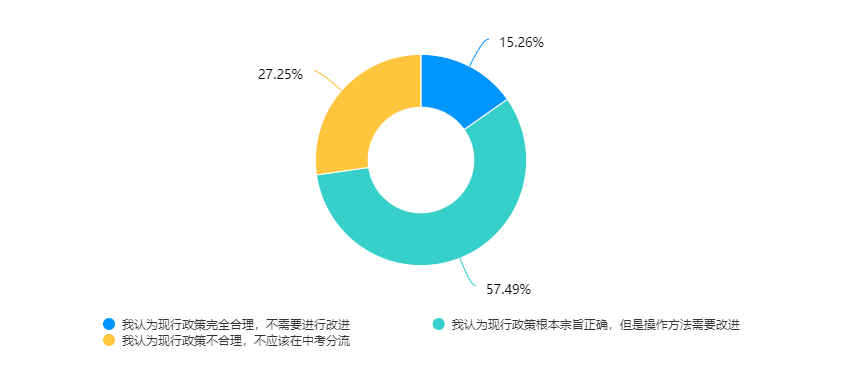
\includegraphics[width=4.6in]{chart/1.png}
	\caption{对中考分流的看法}
	\label{fig:1}
\end{figure}

\par {
	从图 \ref{fig:1} 中容易看出,目前最多的人认为大体正确,但是应当进行一定的改良,这也成为了我们社会实践小组的主要努力方向。
}
\par {
	就此资深英语教师张老师提出了他的中考改革方案,他的话也给了我一定的启发:
	\begin{quote}
		\kaishu
		我赞同的是先缓一缓。而且现在是根据学生的成绩来进行分流,其实最好的情况是根据学生自身的兴趣爱好来进行分流。一直以来通过兴趣爱好来进行人生道路的选择是最有利的。
	\end{quote}
}
\par {
	针对那些认为现行政策完全合理的 112 位受访者,我们询问了他们的详细看法,其结果如表 \ref{fig:2} 所示:
}
\begin{table}[htbp]
	\centering
	\caption{中考分流的优点与合理之处}
	\label{fig:2}
	\begin{tabular}{lcc}
		\hline
		\hline
		{\bf 优势} & {\bf 认同人数} & {\bf 认同比例}\\ \hline
		有助于节省教育资源 & 57 & 50.9\% \\
		有助于优化社会人才结构 & 83 & 74.1\% \\
		有助于提高直接技术本领 & 56 & 50.0\% \\
		有助于环节困难家庭供养学生上学压力 & 21 & 18.8\% \\
		有助于环节就业压力 & 25 & 22.3\% \\
		有助于学生因材施教 & 41 & 36.6\% \\
		\hline
		\hline
	\end{tabular}
\end{table}
\par {
	可以看到,认同中考分流的人主要是因为中考分流可以优化社会人才结构,可以节省有限的教育资源。在研究中我们也会根据这个结果保持分流的优点,扬长避短。
}
\par {
	同时,针对那些认为现行政策完全不合理或者觉得操作方法需要改进的 622 位受访者,我们同样询问了他们的具体意见,其结果如表 \ref{fig:3} 所示:
}
\begin{table}[htbp]
	\centering
	\caption{对改进中考分流方案的看法}
	\label{fig:3}
	\begin{tabular}{lcc}
		\hline
		\hline
		{\bf 改善方案} & {\bf 认同人数} & {\bf 认同比例}\\ \hline
		改善职业教育环境 & 355 & 57.1\% \\
		调整职业教育定位 & 332 & 53.4\% \\
		调整分流比例 & 258 & 41.5\% \\
		调整分流时间 & 192 & 30.9\% \\
		取消中考 & 112 & 18.0\% \\
		其他 & 10 & 1.6\% \\
		\hline
		\hline
	\end{tabular}
\end{table}
\par {
	
	我们对于填选“其他”的人进行了进一步询问,其中有人倡议要建立退出机制,也有人建议高中改为义务制教育。我们认为这过于激进,并不符合社会现状,应该采取折中简介的办法。同样还有一位人士向我们表示,应当像春考一样举行“提前考”,这也和我们拆分为两次考试的方案不谋而合。
}
\par {
	我们针对那些认为应该取消中考的 112
	位受访者产生了一定兴趣,因为取消中考很明显不大为当今教育工作者所接受,我们询问了他们关于取消中考下一步之后的规划,其结果如表 \ref{fig:4} 所示
}
\begin{table}[htbp]
	\centering
	\caption{对取消中考后的方案的看法}
	\label{fig:4}
	\begin{tabular}{lcc}
		\hline
		\hline
		{\bf 新的方案} & {\bf 认同人数} & {\bf 认同比例}\\ \hline
		推行七年一贯制教育(类似上外,浦外) & 14 & 12.5\% \\
		修改学制,推行十年义务制教育(类似上实) & 19 & 17.0\% \\
		实行十二年义务教育 & 78 & 69.6\% \\
		其他 & 1 & 0.9\% \\
		\hline
		\hline
	\end{tabular}
\end{table}
\par {
	
	在他们的案例中,最多人倡导推行十二年义务制教育。对于这一点,相信我们的“高中读一年”方案可以起到一定的作用。当然,也有小部分答卷者选择了修改学制,但无一例外,都认为应当做好初高中衔接,实行某种程度上的一贯制,也有一定的参考意义。
}
\par {
	我们同时还对社会上关心中考分流的朋友做了访谈,前复旦大学学生戚警官表示:
	\begin{quote}
		\kaishu
		进入高中的比例还是要放大。在高中阶段应当建立合适的退出机制,给普通高中的人选择转高职的机会。不该搞一刀切,在初中进行学科类学校和技能类学校的强制分流。
	\end{quote}
	
	如他指出的那样,建立妥当的普通高中退出机制实在是刻不容缓的。目前的一刀切”硬分流“显然不是最优解;从学生的角度来讲:很多聪明的孩子因为家庭条件有限等各种原因被强行分流,着实是非常可惜,是对他们自己和国家的悲剧,应当予以解决。
}

\subsubsection {逐步改进中学课标,搭建完整知识架构}
\par {
	首先,在调查问卷中,我们针对目前的成年人(以及小学生和学龄前儿童)进行了先决调查,即是否了解当前的初中课标课程。调查显示,有 281
	人(50.2\%)选择了是,即了解初中的课程,同时,279 人(49.8\%)选择了否。
	其次,我们针对目前的初高中生以及先决问题中选择了是的受访者进行了进一步调查,询问他们对于当前初中课标课程难易度的看法,结果如图 \ref{fig:5} 与表
	\ref{fig:6} 所示
}
\begin{figure}[!h]
	\centering
	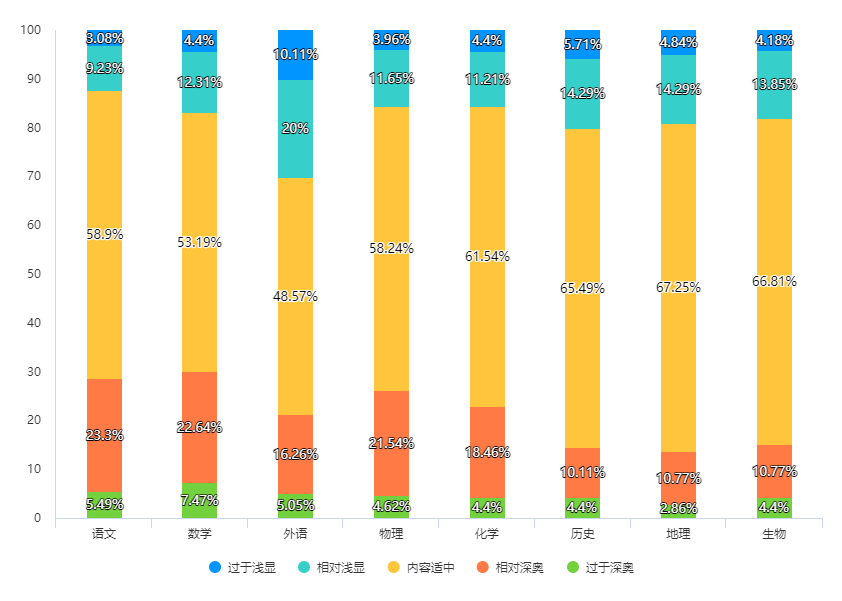
\includegraphics[width=4.6in]{chart/5.png}
	\caption{对各课难度的评价}
	\label{fig:5}
\end{figure}
\begin{table}[!h]
	\centering
	\caption{对各课难度的评价}
	\label{fig:6}
	\begin{tabular}{c|cc|cc|cc|cc|cc|c}
		\hline
		\hline
		\multirow{2}{*}{\bf 科目} & \multicolumn{2}{c}{\bf 过于浅显} &
		\multicolumn{2}{c}{\bf 相对浅显} & \multicolumn{2}{c}{\bf 内容适中} &
		\multicolumn{2}{c}{\bf 相对深奥} & \multicolumn{2}{c|}{\bf 过于深奥} &
		\multirow{2}{*}{\bf 平均分} \\ 
		\cline{2-11}
		{} & 人数 & 比例 & 人数 & 比例 & 人数 & 比例 & 人数 & 比例 & 人数 & 比例 & {} \\ \hline
		语文 & 14 & 3.08\% & 42 & 9.23\% & 268 & 58.90\% & 106 & 23.30\% & 25 & 5.49\% &
		3.19 \\
		数学 & 20 & 4.40\% & 56 & 12.31\% & 242 & 53.19\% & 103 & 22.64\% & 34 & 7.47\%
		& 3.15 \\
		外语 & 46 & 10.11\% & 91 & 20.00\% & 221 & 48.57\% & 74 & 16.26\% & 23 & 5.05\%
		& 2.85 \\
		物理 & 18 & 3.96 \% & 53 & 11.65\% & 265 & 58.24\% & 92 & 21.54\% & 21 & 4.62\%
		& 3.11 \\
		化学 & 20 & 4.40\% & 51 & 11.21\% & 280 & 61.54\% & 84 & 18.46\% & 20 & 4.40\% &
		3.07  \\
		历史 & 26 & 5.71\% & 65 & 14.29\% & 298 & 65.49\% & 46 & 10.11\% & 20 & 4.40\% &
		2.93  \\
		地理 & 22 & 4.84\% & 65 & 14.29\% & 306 & 67.25\% & 49 & 10.77\% & 13 & 2.86\% &
		2.93  \\ 
		生物 & 19 & 4.18\% & 63 & 13.85\% & 304 & 66.81\% & 49 & 10.77\% & 20 & 4.40\% &
		2.97  \\ \hline
		{\bf 小计} & 185 & 5.08\% & 486 & 13.35\% & 2184 & 60\% & 609 & 16.73\% & 176 &
		4.84\% & 3.03  \\ 
		\hline
		\hline
	\end{tabular}
\end{table}
\par {
	
	从中我们根据柱形图和表格当中的平均数可以发现,对于课程内容难度的评分(其中过于浅显为1分,过于深奥为5分)基本呈现正态分布,但相较于其他学科,语文和理科的学科普遍表示难度较高。
}
\par {
	首先,关于理科,南京外国语的 Z 同学表示:
	\begin{quote}
		\kaishu
		我的切身体会就是感觉初中有一些毫无意义的抄写作业,还有理科(特别是数学)做了太多无意义的简单题,导致考试的时候一些稍微难、新一点的题很多同学(包括我)会停顿甚至做不出来。换句话说,感觉初中文化课对思维提高的锻炼和引导还不够。
	\end{quote}
	同时,问卷中也有人补充到:
	\begin{quote}
		\kaishu ……另外,数学没有必要一定按照步骤(注:即特定的思路套路)去做,这样发挥的思路少了,比较局限。\\
		中国的教育往往注重方法不注重方法是怎么来的,教出来的学生可能不具有足够的举一反三能力。
	\end{quote}
	
	从中我们可以看出,理科对于思维的锻炼和引导需要加强。过于注重套路化,不仅对于初中的学习和考试,实质上对初高的衔接也有影响。而我们在日常的学习中也应该注重对思维的锻炼。
}
\par {
	
	我们再来分析一下语文。我们针对填写了“过于深奥”的受访者进一步询问他们的理由,其中包括:语文学习逻辑性弱,每个人对阅读的理解不同,希望能增加语文答案的客观性等想法:
	\begin{quote}
		\kaishu
		阅读分析选择题经常有争议,要是学生比出题老师更能理解选文作者的意思呢?要出就出客观一点的,有绝对真理的;语文是灵活的,标答的存在本身就是一个错误的存在。每个人对阅读的理解不同,强制背下的标答有何意义?
	\end{quote}
}
\par {
	针对这一现象,我们向一位在崇明区从事三十年语文教育的高级教师询问,应该如何帮助学生解决语文学习的问题,他给了我们如下的建议:
	\begin{quote}
		\kaishu 语文主要是多读文章,多读古文。书读百遍其意自现。别的学科都有异曲同工之妙。多读读自然就能培养兴趣。
	\end{quote}
	由此可见,针对此现象,我们需要认识到“多读”一直是语文的一个重要学习方法。
	我们也询问了董涛玲老师关于现在语文出题的想法:
	\begin{quote}
		\kaishu
		语文现在的出题方向趋向于思维品质,但是中考的语文的选拔性仍然稍弱。现在语文考试做的比较好的地方在于注重了语文素养,但是做的不够的地方差异性也比较小,相当一部分的学生通过纯刷题能得到令人满意的结果。中考语文的思辨性,批判性思维和高中有很大的差距,有提高空间。
	\end{quote}
}
\par {
	同时,我们也采访了所有的成年人,询问了他们关于当时初中课程的难易程度,其结果同现在大致相似,如图 \ref{fig:7} 和表 \ref{fig:8} 所示。
	
}
\begin{figure}[!htb]
	\centering
	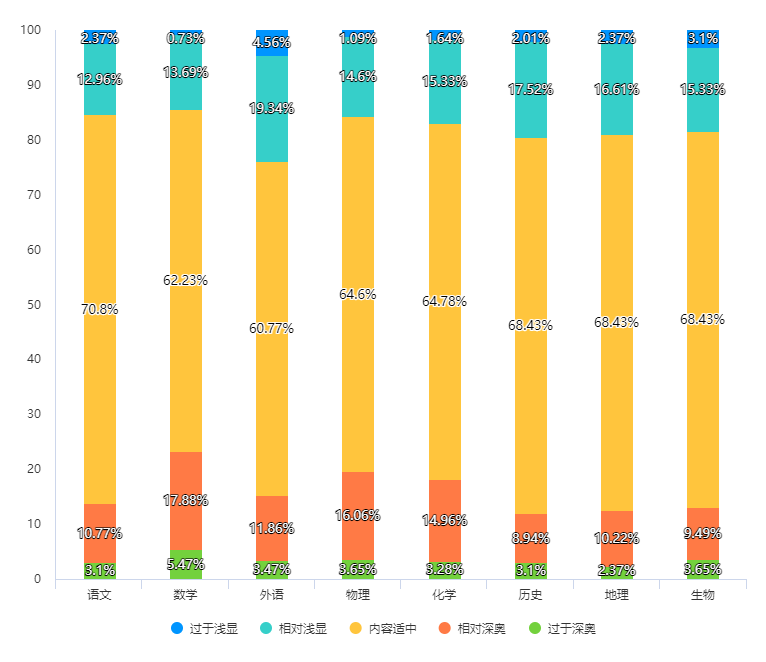
\includegraphics[width=4.6in]{chart/7.png}
	\caption{对曾经的各课难度的评价}
	\label{fig:7}
\end{figure}
\begin{table}[!htb]
	\centering
	\caption{对曾经各课难度的评价}
	\label{fig:8}
	\begin{tabular}{c|cc|cc|cc|cc|cc|c}
		\hline
		\hline
		\multirow{2}{*}{\bf 科目} & \multicolumn{2}{c}{\bf 过于浅显} &
		\multicolumn{2}{c}{\bf 相对浅显} & \multicolumn{2}{c}{\bf 内容适中} &
		\multicolumn{2}{c}{\bf 相对深奥} & \multicolumn{2}{c|}{\bf 过于深奥} &
		\multirow{2}{*}{\bf 平均分} \\ 
		\cline{2-11}
		{} & 人数 & 比例 & 人数 & 比例 & 人数 & 比例 & 人数 & 比例 & 人数 & 比例 & {} \\ \hline
		语文 & 13 & 2.37\% & 71 & 12.96\% & 388 & 70.80\% & 59 & 10.77\% & 17
		& 3.10\% & 2.99\%  \\
		数学  & 4 & 0.73\% & 75 & 13.69\% & 341 & 62.23\% & 98 & 17.88\% & 30 & 5.47\% &
		3.14  \\ 
		外语 & 25 & 4.56\% & 106 & 19.34\% & 333 & 60.77\% & 65 & 11.86\% & 19 & 3.47\%
		& 2.90 \\
		物理 & 6 & 1.09\% & 80 & 14.60\% & 354 & 64.60\% & 88 & 16.06\% & 20 & 3.65\% &
		3.07  \\
		化学 & 9 & 1.64\% & 84 & 15.33\% & 355 & 64.78\% & 82 & 14.96\% & 18 & 3.28\% &
		3.03  \\
		历史 & 11 & 2.01\% & 96 & 17.52\% & 375 & 68.43\% & 49 & 8.94\% & 17 & 3.10\% &
		2.94 \\
		地理 & 13 & 2.37\% & 91 & 16.61\% & 375 & 68.43\% & 56 & 10.22\% & 13 & 2.37\% &
		2.94  \\
		生物 & 17 & 3.10\% & 84 & 15.33\% & 375 & 68.43\% & 52 & 9.49\% & 20 & 3.65\% &
		2.95  \\ \hline
		{\bf 小计} & 98 & 2.24\% & 687 & 15.67\% & 2896 & 66.06\% & 549 & 12.52\% & 154
		& 3.51\% & 2.99  \\
		\hline
		\hline
	\end{tabular}
\end{table}
\par {
	我们同样针对填写了“过于深奥”的受访者进一步询问他们的理由,其中包括:学习的内容应该更加贴近生活,而不是为了答题而答题,和采用国际化的考试标准等。
}
\newpage
\par {
	
	有一些朋友认为,应当和生活实际相联系,而不是脱离实际的”强行答题“。这种意见也很有代表性,我们在接下来的社会实践部分会提供解决方案着重消灭这个问题。当然,也有一部分受访者认为初中的课表过于简单,他们认为:
	\begin{quote}
		\kaishu 外省市的很多知识上海删掉了,我认为理科应当和外省市看齐。\\
		\sout{陆老师的课太简单了(我们也不知道这位问卷作答者是谁)。}
	\end{quote}
}
\par {
	在这些意见中,
	我们发现,基础课程,特别是以数理化为代表的科学性课程,其课程安排在初中阶段相对独立,和高中没有合适的接轨,无法完整地形成一个体系。这就导致高中课程本身的课程内容产生跳跃性,在具体学习会有片段感。
}
\par {
	
	为了解决这些问题,我们通过与不同学校学生进行交流,最终得到一个结论:我们需要改革当前的课程标准,给予学生一个知识架构完整的课程体系,保证学生在初中与高中过渡时不会出现难度的落差感以及知识点的错位。
}
\par {
	根据这个结论,我们结合新课标提出一个改善方案。这个方案主要由两部分组成:将教师的教学内容连贯化,将教师的教学方式区分化。
}
\par {
	
	通过将教师的教学内容变得更加连贯,我们要对课程本身的初高衔接做改动。以现行的数学教材作为例子分析,初中阶段的最后部分是几何的计算和证明的内容,而高中部分的第一章是集合与逻辑的内容,两者之间几乎没有关联性,后者在初三课程中也没有铺垫课程的设置。另一个案例是目前的化学课程,初中阶段学习的虽知识面然相对较广,但是没有解释实验现象背后的原理,导致我国化学高中课程需要从头开始,从原子的结构入手对初中的知识进行解释,甚至出现了“在初中这个知识点是错的,到了高中就变成对的”的奇异现象。
}
\par {
	
	在“高中读一年”的综合方案下,这种种不合理的会被缓解。通过对于现有框架进行专题化处理,每一个知识点模块化地教授,而不是分散地散落在课程设置的不同角落,避免教学内容在不同学段自相矛盾的情况,从而构建正确的知识体系。
}
\par {
	
	在缓解初三第二学期集中复习“内卷”的背景下,开展初高衔接教学,及时地引入高中课程,最大幅度地减少因为学习内容不适应导致心理落差,出现成绩波动较大的现象。消除了这些因素的干扰,“高中读一年”中考察学生对于学习方式改变的部分能够更为客观,也为高中一年级期末考试的分流得出更加科学的结果。
}
\par {
	
	从教学方式区分化的角度入手,因为初高中的知识在难度上和结构有本质性的不同,所以必须采用不同的教学手法,这一点也要予以改革。正是因为这种不可避免地教学方法的调整,所以会导致部分同学不适应高中学习生活。普通高中的退出机制寻求解决这一问题。通过一场考试帮助那些有学习动力的中专生上升至普通高中,帮助不适应高中生活的同学退出去中专学习职业技能。至于如何让我们能够尽快地适应高中的模式,班主任陆老师指出了明路:
	\begin{quote}
		\kaishu 保持好良好的学习态度和学习方法,加上自己的调整要达到高中学段的基本学习要求还是没什么困难的。
	\end{quote}
}
\par {
	因此,构建合理的知识体系,寻得合理地学习方法,组织合理的学习逻辑,即能适应高中学制下的学习压力,实现更有效率,更有价值的教育 。
}

\subsection {社会多方通力合作保障总和素质评价系统落地}
\par {
	
	为了保障综合素质评价系统在全市范围内的有效实施,避免出现流于形式,社会各方面不重视等负面现象。我们计划通过各种手段方法来引起社会重视,提高学生在社会实践活动中的参与感和体验感。我们从“品德发展和公民素养”“探究实践和创新能力”这两个角度入手研究。
}
\par {
	
	从“品德发展和公民素养”即学生的社会实践能力来看,我们第一计划做好学校和社会力量的联动,充分调动社会资源,在全市范围内增设社会实践站点;第二完善社会实践参与人员的招生制度,增加实践课题的多样性,让每个学生都找到真正适合自己的社会实践内容;第三建议学校在做出全校的社会实践安排同时,给予学生一定的假期,同时做好相关学校政策的安排,为家长老师参与进社会实践活动提供便利,创造条件;最后,在做出实践活动的安排下,应当充分咨询各方面的意见,实现“因材施教”。
}
\par {
	
	从“探究实践和创新能力”即青少年的创新实践水平来看,我们第一计划将创新研究的课题与新课程标准相挂钩,避免泛泛而谈,转而深入研究一个课题;第二增设“少科站”一类的创新实践基地,让普通学生有更多机会接触利用公有资源;第三调整评价模式,不能只考察书本知识,应当多多培养团队协作和动手能力。
}

\subsubsection {民间力量和公有资源结合,提高社会实践活动质量}
\par {
	
	首先,通过前面浦外的张同学的例子我们可以发现,如今有意愿参与社会实践的同学难以通过简易的通道参与优质的活动。据此,我们提出:民间力量和公有资源应当有更加有效的合作。先,根据现有的访谈和问卷资源,我们对他们进行整合和归纳,提炼出有价值的观点和建议。
}
\par {
	首先,我们询问了大家对当前综合素质评价系统的了解程度,结果显示,有56.81\%的答卷者对综合素质评价系统有一定的了解,体现出社会对素质教育的普遍关心。
}
\par {
	接下来,我们询问社会实践在初中开展是否有必要,结果如图 \ref{fig:9} 所示:
}
\begin{figure}[!htb]
	\centering
	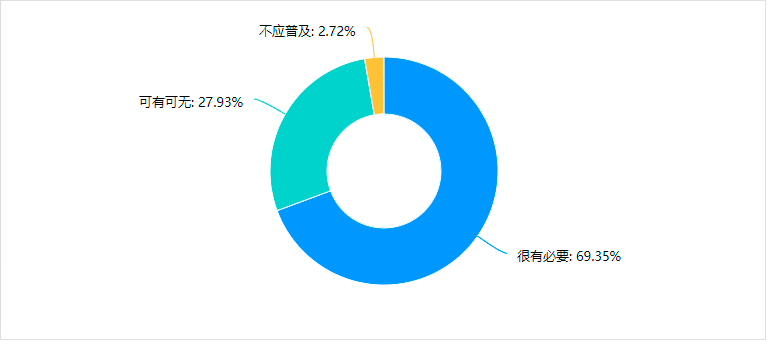
\includegraphics[width=4.6in]{chart/9.png}
	\caption{对社会实践必要性的调查}
	\label{fig:9}
\end{figure}
\par {
	从环形图中可以看出,绝大部分的人群都认为应当存在社会实践,其中认为“很有必要”的更是占了多数。这也正是我们努力的方向,把社会实践做的更有意义和价值。
}
\par {
	当然,世界上并不存在完美的事物,万物都存在一定的弊病。针对这一现象,我们询问答卷者他们所认为社会实践存在的缺点,如表 \ref{fig:10} 所示:
	\begin{table}[htbp]
		\centering
		\caption{现有社会实践方案的问题}
		\label{fig:10}
		\begin{tabular}{lcc}
			\hline
			\hline
			{\bf 问题} & {\bf 认同人数} & {\bf 认同比例}\\ \hline
			流于形式 & 528 & 71.9\% \\
			未能普及,极少人关注 & 471 & 64.1\% \\
			学生不重视,不了解该方案或学校已经帮助填报完成 & 294 & 40.1\% \\
			老师不重视,完全不或极少提供帮助 & 205 & 27.9\% \\
			家长不重视,认为占据过多时间并影响正常工作 & 254 & 34.6\% \\
			其他 & 20 & 2.7\% \\
			很好,没有问题 & 45 & 6.1\% \\
			\hline
			\hline
		\end{tabular}
	\end{table}
}
\par {
	从表格中可以发现,最严重的问题莫过于担心社会实践流于形式。此外,从老师,家长,学生不重视的角度来看,各有一批人认为缺乏重视和必要的资源。此外还有一些其他意见:
	\begin{quote}
		\kaishu 实践总时间过长,不考虑学生课余时间能否完成。没有人能认真完成,流于形式,应付了事。\\
		需要家庭投入大量时间支持,学生课业负担较重,考核不降低,社会实践变相增加负担。\\
		实操性太差,初中考试考级科目较多,课业负担较重,几乎没有空余时间。社会实践的项目较少,大多是走个过场。\\
	\end{quote}
	
	以上意见,主要表达了对学生,家长时间不够的担忧。稍后会在第三个建议中解决这一问题。有人提议设立奖励机制,将其作为一个较为重要的成绩去看待,但是问卷的一些回答表现出了强烈的反对:
	\begin{quote}
		\kaishu
		作为义务教育阶段,社会实践,特别是普遍的社会实践,势必会给各家庭带来一笔经济支出,且社会实践内容五花八门各不相同,便会出现三六九等,大概有一些利用资本购买教育资源的嫌疑吧;当然这么说一切的前提都是社会实践不仅仅是综评的必要的评价因素之一,且真正的有一定的“奖励机制”,会实际的影响初中生的升学。
		\kaishu 容易被权贵利用进行弹性操作,更可能产生利益链之下的产业化操作,易生猫腻,与初衷背道而驰。
	\end{quote}
	
	以上意见主要表达了对“黑幕”“权贵操弄”的担忧,这种评价机制我们也是要竭力避免的。当代青年人固然缺乏必要的实践,然而容易产生“开后门”“弹性操作”等不良现象,所以“素质教育”是很难加以量化的,倘若量化就可能会变质。假如冒然综合素质评价体系纳入中高考等评价体系与升学挂钩
	,只会导致不公开不透明的黑幕。
}
\par {
	这种“黑幕”的典型案例就是父母时代的“国家三好学生”的评比\footnote{《共青团中央
		教育部关于表彰“全国三好学生”、“全国优秀学生干部”和“全国先进班集体”的决定》\url{http://www.moe.gov.cn/jyb_xxgk/moe_1777/moe_1779/201007/t20100722_92927.html}}。戚若渝同学的母亲就是”国家三好学生“高考加分政策的受益者,她表示:
	\begin{quote}
		\kaishu
		所有接轨进评价系统的主观加分都制造不公平。当时我是靠“国家三好学生”高考加了三十分。你说这个“国家三好学生”的荣誉那里来的?真的公开公平嘛?当时还是靠大奶奶找上海教育局的人把崇明唯一的两个名额中留了一个给你妈。
		所以这种办法行不通。
	\end{quote}
	因而可见,这种办法实在是不妥当的。
}
\par {
	然后,我们再看一下对社会实践具体形式的批评。前崇明中学党委副书记郭老师提出了想法:
	\begin{quote}
		\kaishu 毛主席说不能脱离群众,现在很多年轻人就有点脱离群众。假如你们多做一点职业体验社会实践,就会意识到读书的重要性。
	\end{quote}
	问卷中也有很多人表现出了相同的顾虑:
	\begin{quote}
		\kaishu
		社会实践,以前说是学工学农,我觉得很好,现在太过形式,对于小朋友而言,社会实践可能就是去去科技馆、博物馆。不能说有问题,但是四肢不勤五谷不分的问题还是存在。\\
		应当引导学生用心观察社会需求,做一些力所能及的真正对社会有意义的事情,而不是教会他们做表面功夫。\\
		学校组织的社会实践无非两种:学农/军训或春秋游,我觉得春秋游不应止于玩乐,可以抽出半天参加一些志愿者或义工,哪怕在旅游地点捡些垃圾美化环境。\\
		因为并不了解社会实践所以并不能发现什么问题。\\
	\end{quote}
}
\par {
	接下来,我们从“学生不重视”“家长不重视”“老师不重视”三个维度进行了进一步调查,希望能为发现方案提供一些灵感和思路。对于学生不重视的 294
	人,调查结果如表 \ref{fig:11} 所示:
	\begin{table}[htbp]
		\centering
		\caption{对学生不重视的解决方案}
		\label{fig:11}
		\begin{tabular}{lcc}
			\hline
			\hline
			{\bf 解决方案} & {\bf 认同人数} & {\bf 认同比例}\\ \hline
			将社会实践成绩纳入学生档案 & 133 & 45.2\% \\
			在一定范围内对表现积极,成绩优异者开展全面表彰 & 151 & 51.4\% \\
			做好宣传工作,普及价值和重要性 & 163 & 55.4\% \\
			设立相关服务站点,走进普通学生生活 & 146 & 49.6\% \\
			提高社会实践质量,吸引同学参加 & 212 & 72.1\% \\
			举办丰富多样的交流评比,调动积极性 & 128 & 43.5\% \\
			其他 & 7 & 2.4\% \\
			\hline
			\hline
		\end{tabular}
	\end{table}
}
\par {
	
	可以发现,大家最关心的问题是“提高社会实践的质量”。对于比较有争议的“纳入学生档案”和“交流评比活动”则支持率不高。设立服务站点也得到了一定的支持。有一位朋友在题目下面的留言,相信说出了不少家长朋友的心声:
	\begin{quote}
		\kaishu
		社会实践应是自发的、有内在动力的。不同学生的兴趣和能力领域不同,效果好的社会实践项目也不同。强制性的社会实践是无意义的,况且你瞧瞧现在这社会能有几种实践形式啊。
	\end{quote}
	我们要调动积极性,尽量避免避免强制性的社会实践,同时丰富社会实践的课题,给予自由的形式选择。
}
\par {
	对于选择老师不重视的 205 人,调查结果如表 \ref{fig:12} 所示:
	\begin{table}[htbp]
		\centering
		\caption{对老师不重视的解决方案}
		\label{fig:12}
		\begin{tabular}{lcc}
			\hline
			\hline
			{\bf 解决方案} & {\bf 认同人数} & {\bf 认同比例}\\ \hline
			做好宣传工作,让老师了解其必要性 & 101 & 49.3\% \\
			改善社会实践安排,使其更具教育价值 & 140 & 68.3\% \\
			组织老师走进场馆,切身体会社会实践 & 123 & 60.0\% \\
			指导学生社会实践纳入老师正常工作量 & 138 & 67.3\% \\
			将社会实践学生结果纳入职称评选系统 & 105 & 51.2\% \\
			其他 & 7 & 3.4\% \\
			\hline
			\hline
		\end{tabular}
	\end{table}
	
	可见,关于“纳入正常工作量”和“改善社会实践安排”,支持的朋友比较多。大家也同意在工作量不增加的前提下丰富老师的工作安排。对于有争议的“纳入职称评选系统”和较为形式的“做好宣传工作”,支持率相对并不高。有一位答卷者还提出:
	\begin{quote}
		\kaishu 现在的老师又有多少经历过社会实践,不同的实践应该有不同的老师担任,担任者不应只存在于学校。
	\end{quote}
	可见,老师的专业性和社会资源的运用也是大家关心的议题。所以,运用民间力量和共有资源也可见一个重要的解决方法。
}
\par {
	对于选择家长不重视的 254 人,调查结果如表 \ref{fig:13} 所示。
	\begin{table}[htbp]
		\centering
		\caption{对家长不重视的解决方案}
		\label{fig:13}
		\begin{tabular}{lcc}
			\hline
			\hline
			{\bf 解决方案} & {\bf 认同人数} & {\bf 认同比例}\\ \hline
			开展宣传工作,向中小学家长普及社会实践必要性 & 134 & 52.8\% \\
			活动场馆调整方案,鼓励家长与孩子共同完成社会实践 & 138 & 54.3\% \\
			做好家校联动,以学校为平台促进亲子互动 & 167 & 65.8\% \\
			推行公有化的社会实践机构,使学生更好走进社会活动 & 167 & 65.8\% \\
			各大企事业单位能够提供一些时间的假期来推动家长学生一起实践 & 147 & 57.9\% \\
			其他 & 9 & 3.5\% \\
			\hline
			\hline
		\end{tabular}
	\end{table}
	
	从中我们可以发现各个选项的支持率较为平均,如“做好家校联动”,“推动公有化的社会实践机构”“提供一些假期”等方案有较高的支持率。我们会在方案中体现这几点。从具体的留言中,我们筛选了比较典型的进行分析。
	\begin{quote}
		\kaishu
		企事业、实践机构提供平台和有趣、有意义的实践活动,对承办计划实践活动的企业予以一定支持(社会面或经济面,提供假期或提供实践活动的企业可以得到一些奖励或补偿)。
	\end{quote}
	这样的方案也能一定程度上解决家长工作繁忙无法顾及的问题。
}
\par {
	最后,在留言板块中,一位问卷中的朋友点出了社会实践成功的必要条件:
	\begin{quote}
		\kaishu
		不过,在我看来,是社会实践制度也是可行的,关键就在于学生能否真正成为认可喜爱社会实践,学校是否认可,家长是否支持,社会是否接受,能不能成为一种学生文化。如若可以,我觉得绝对可以大幅提高中国学生素质。
	\end{quote}
}
\par {
	据此,为了提高社会实践活动质量,我们提出四个意见:
	\begin {itemize}
	\item [1)] \textbf{做好学校和社会力量的联动,充分调动社会资源,在全市范围内增设社会实践站点。}
	\par {
		在访谈过程中,有家长向我们指出,应当更好地利用公有资源,使其发挥作用:
		\begin{quote}
			\kaishu 国家整合资源去做的免费资源,为什么不利用?让孩子亲身体验,接触这种学习资源。学习不能拘泥于课本,这是多元化学习中的重要一环。
		\end{quote}
		我们询问了资深英语教师张老师,他为我们提出了一个相对合理的建议:
		\begin{quote}
			\kaishu
			做好社会实践需要学生社会学校家长四方面一起重视的。这样至少对学生某一方面的素质是有很打提升的。这其中最为重要的就是社会层面,应当由社会出发,给予学生一个充分的平台来施展他们的才能。
		\end{quote}
		上大附中实验学校的金老师也表达了相似的观点:
		\begin{quote}
			\kaishu
			现在的社会实践实在是十分流于形式,必须要让学校和家长联动起来,帮助学生去获取一些社会当中的资源,让学生能够充分的利用到这些资源,不然的话学生的社会实践最终就沦为了参观博物馆,完全对于他们的成长没有任何的帮助。
		\end{quote}
		
		根据这一点,我们欣喜地发现,上海市教育部门已经在着手建立社会实践基地了。社会实践基地是经各级政府校外教育活动联席会议办公室登记确认,为学生提供社会实践活动的学习场所。以上海市为例,目前遴选出来的市级场地有
		93 个\footnote{易臻真,王洋,2019,中国教育学刊
			\url{https://kns.cnki.net/kcms/detail/detail.aspx?dbcode=CJFD&dbname=CJFDLAST2019&filename=ZJYX201905022&uniplatform=NZKPT&v=qwGZA0S2sEptdaQGQhwkNCaEg3UWgH21C-gH5-0gpW-3qo_HkOvH9L2cYDoOiqeD}}。上海市市场监督管理局每年都会增设一批新的社会实践基地,也是这一行为的一大例证。我们希望以此为基础,增加基地数量,保证学生能够更加便利地在认证地点开展活动。
	}
	\item [2)] \textbf{改善社会实践在实践主题多样性。}
	\par {
		
		在艺术音乐、社会科学、自然科学等不同方面举办丰富多彩的活动。可以尝试让校方直接和企业接洽,缓解社会实践项目依赖家长的资源这一现状。我们在访谈中发现,很大一部分同学不愿意参加或者不喜欢社会实践活动的原因就是因为活动死板,没有多样性。活用社会资源,给予学生更多的实践的选择自由度,可以更好地解决这个问题。尽管并不多的学校能有像上外附中的长时间自主实践,我们仍能在一定范围内提供多样化的选择。南京外国语学校的
		Z
		同学向我们分享了他们的模式:在家长群中进行各类社会实践的分享,并让家长和学生讨论后组团报名获取积分。这样的模式在提供多样化的选择的同时,“组团参加活动”也符合学生们的社交需求,调动积极性。Z
		同学表示:
		\begin{quote}
			\kaishu 同学们普遍看好这种活动,因为其实无论怎么都是有收获的,尤其是能和同班同学一起实践。
		\end{quote}
	}
	\item [3)] \textbf{企事业为家长帮助学生社会实践提供更好的条件。} 
	\par {
		
		我们从问卷和访谈中发现,不少同学家长无法进行社会实践,归根结底是客观时间因素阻碍。建议学校在做出全校的社会实践安排同时,同时做好相关学校政策的安排,为家长老师参与进社会实践活动提供便利,创造条件。家长所工作的企业也应当安排适当的休假,协助他们参加孩子的实践活动。指导老师董涛玲告诉我们,这点在学校已有体现:只要和工作安排不冲突的,学校每个月都为教师应当提供适量的假期,为家长参与社会实践活动提供便利,创造条件。
	}
	\item [4)] \textbf{充分听取学生与家长的意见}
	\par {
		
		我们在访谈中发现,存在一些开展强制性“兴趣班”的学校。对此,我们提议,如果校方选择开展要求所有学生参加的活动,对于活动内容就应该有更加细致入微的甄别和选择。我们希望学校在做出决定前应当聆听学生和家长的意愿和想法,再得出一个能让多数人满意的结果,“画出最大同心圆”。倘若一味地要求所有学生参与此类活动终究有强人所难之嫌,只有用因材施教的办法去让学生选择自己喜爱的项目进行学习才能达到社会实践培养“探究和创新精神”这一应有之义。
	}
	\end {itemize}
}
\par {
	最后,我们想要给出一个具体的操作方案来增加方案的可行性。在这一点上,南京的素质评价系统对我们很有启发。我们对其进行了较为深入的研究,提出我们自己的方案:
}
\par {
	
	我们建议,给每位同学们发一个公益积分册,每学期需要做一定量的公益活动,对校内的公益活动应当设置上限避免学校集中组织形式主义活动”水积分“。这样就能完善评价机制,避免“流于形式”的现象发生。
}
\par {
	
	我们计划,以学校为单位建立一个公益群,然后通过学校和民间企业对接,定期找公益活动发到群里,家长可以用接龙的方式给为孩子报名活动。这也是我们“民营资源和公有力量相对接”的灵魂思想和生动体现。主办方在活动结束后开积分条证明同学在这一段时间进行了该公益活动。这也是一种完善评价机制的手段。
}
\par {
	我们要推动主题的多样化,推出一些大家喜欢的,对社会有益的社会实践项目,例如去一个科技展去教别人体验 VR
	科技等。同时我们要为教师和家长提供一定的假期,在不妨碍正常工作的前提下给他们时间资源参与到孩子的社会实践中。这种模式是公有资源和民营企业深度合作的典范,是同学们自主选择课题的典范,是充分协商后进行高价值社会实践的典范。
}




\subsubsection {运用政策工具与教学机制,发展创新实践能力水平}
\par {
	正如前文所述,当前青少年缺乏创新精神能力是为世人同意的观点,为了解决这方面的问题,我们在调查问卷中对受访者询问了他们对于改进的建议,结果如图
	\ref{fig:14} 所示:
	\begin{table}[htbp]
		\centering
		\caption{对缺乏创新精神的解决方案}
		\label{fig:14}
		\begin{tabular}{lcc}
			\hline
			\hline
			{\bf 解决方案} & {\bf 认同人数} & {\bf 认同比例}\\ \hline
			鼓励学生突破学校学习,突破自我 & 496 & 67.6\% \\
			使教学方式更加灵活多变,层次分明 & 522 & 71.12\% \\
			开展宣传工作,让学生们体会其重要性 & 286 & 39.0\% \\
			线下设立创新实验基地,聘请专业老师指导 & 462 & 63.0\% \\
			重新设计相关教材,更加灵活多变,使学生寻得兴趣 & 459 & 62.5\% \\
			其他 & 24 & 3.3\% \\
			\hline
			\hline
		\end{tabular}
	\end{table}
	在“其他”中,有不少朋友给我们留言,我们从中遴选了有价值的发言供大家参考:
	\begin{quote}
		\kaishu
		我很赞同学习是自己的事,这里的“学习”就包括了课外学习。因此当你把课内学习与课外学习割裂开来、还要反过来通过学校宣传课外学习时,就说明学校眼中的课外学习是失败的,而促成了这一点的它还要为所谓素质教育、综合发展做个形式。想解决课外学习浅薄的问题,只有从课内学习占比太大的病根下手。\\
		不要只重视分数而不重视每个人独有的天赋,这个和家庭的观察和老师的培养密不可分。\\
		教育设施要跟上,学科要开发完善而且广泛。\\
	\end{quote}
}
\par {
	首先,从中我们可以发现,改变当前教育形式,使教育形式灵活多变是最为热门的选择答案。就读于 MIT 的金学长告诉了我们初中培养学科兴趣的重要性:
	\begin{quote}
		\kaishu
		对一个初中生来说,许多学科都是人生中第一次学,那么这样子的话老师讲的课上的内容就是这个学生对这门学科的第一印象。然后这个就会很影响学生对这门学科总体的兴趣。比如我初中的时候感觉物理和化学都不如数学有意思。但后来大学时接触了一些物理,就完全不是一个感觉,非常有意思。然而那时候即使有兴趣也已经没有精力去学了。
	\end{quote}
	同时,将学生探究重点与学校内容有机结合,而不是针对社会上的一堆热门新闻泛泛而谈也是一个必不可少的过程,例如批判性思维,资深英语辅导教师叶叶这样表示:
	\begin{quote}
		\kaishu 我认为应当培养Critical thinking:
		即理解的情况下从中立多方面给出答案,需要搜集信息和看书。我不赞同碎片化信息,书都是经过审核的不存在虚假信息所以可以阅读来增长见识。过程是:积累知识,提出问题,开设课题。注意:需要有有学术能力的老师进行指导。
	\end{quote}
	
	陆老师给出了他在培养学生兴趣方面的经验。
	\begin{quote}
		\kaishu 从小接触的教育,对一个大方向产生兴趣,随着成长中不断尝试不断收获的过程,将这个范围逐渐缩小,直到找准对某一个学科的探究性兴趣。
	\end{quote}
	我们可以看出,探究性兴趣的培养不能是一直广撒网,而是应该慢慢缩小范围并且“放长线钓大鱼”,针对一个有价值的课题进行深入的研究,只有这样才是真正的探究性精神。
}
\par {
	
	综合来看,家长们和老师们普遍认为创新实践能力非常重要,但是在当代年轻人中相对匮乏。学校课程设置上面仍然拘泥于照本宣科,没有走向社会的环节。其中比较典型的代表莫过于崇明中学党委副书记郭老师提出的提高创新实践能力的办法:
	\begin{quote}
		\kaishu 创新都是从生产活动中迸发出来的,要亲自参与到一线劳动中,才能培养创新精神呀,否则只会流于形式,形而上学。
	\end{quote}
}
\par {
	在此基础上,在2019年发表于中国教育学刊上的《城市高中社会实践活动课程长效机制的构建探索
	———以上海市曹杨第二中学为例》\footnote{易臻真,王洋,2019,中国教育学刊,\url{https://kns.cnki.net/kcms/detail/detail.aspx?dbcode=CJFD&dbname=CJFDLAST2019&filename=ZJYX201905022&uniplatform=NZKPT&v=qwGZA0S2sEptdaQGQhwkNCaEg3UWgH21C-gH5-0gpW-3qo_HkOvH9L2cYDoOiqeD}}一文中,详细说明了现在的社会实践缺乏系统的课程设计及反馈评估机制,且各级政府相关政策不够细化难以落实,并提出了加强城市高中社会实践基地的遴选工作,完善城市高中社会实践活动课程的申报机制,落实城市高中社会实践活动课程的手册编制工作,提升城市高中社会实践课程的自我更新能力等多项建议。
}
\par {
	
	关于如何建立评价机制,该文章也做出详尽的建议,其中有几点和我们不谋而合。他强调:我们要关注活动设计的针对性,更要关注学生在活动中有效性结果的生成过程。我校英语教师陈老师分别以家长和老师两个身份提出自己的看法,为我们提供了思路:
	\begin{quote}
		\kaishu
		作为家长,我觉得如果一个小组想要做到最好,那家长也需要分工,力所能及地帮到学生当然是好的,但是还是希望学生能够自主完成;作为老师,想要让社会实践能够和校内课程结合起来的话,就需要硬性地指定一些课题,这样学生们都可以比较深入地钻研一个话题,而不是像很多现在的课题,对于一个时事热点泛泛而谈。
	\end{quote}
}
\par {
	经过总结,我们从三个方面提出了建议:
}
\begin{itemize}
	\item [1)] 促使课标内的单元课题成为社会实践选题的主流。
	\par {
		
		这样既做可以抬高实践的深度,但又不增加相应的难度。现在的社会实践注重于发现生活中的小问题,并以此为切入点挖掘。这样做确实能够对于学生的周遭有更深刻的认识,但同时考验学生具备的学术能力。很多专业性内容需要从头学起,而这对于一个学生相对有限的时间来说太过紧迫。以不同在校学习的学科为基础设置选题范围,既可以满足不同学生的学术需求,也可以降低学习成本,使重点落回“实践”中。同时,这对于课内知识的创新研究也是有益处的,正如上海知名信息学竞赛教练马融在访谈中所说:
		\begin{quote}
			\kaishu
			提升探究性兴趣,需要有这门学科跟日常生活或者说学生能接触到东西的关系。从能接触到的问题出发,然后看这个学科对这个生活实践的帮助,那么这样子呢,这个学生搞探究会比较有热情。
		\end{quote}
	}
	\item [2)] 多发运用社会资源和民间力量。
	\par {
		
		我们的既然学校与家长方面较难做到有效的辅导学生培养创新精神,我们在前文提出使用民间力量和公有资源与社会实践的结合的办法,一方面可以节省家长的精力,一方面可以使学生实践时有更高的自主性。我校在2020年1月正式与中科院上海天文台合作共建签约,便是公有资源和民间力量,学校和社会团体密切合作的正面案例。
	}
	\item [3)] 调整综合素质的评价模式。
	\par {
		我们希望能够调整评价模式,不能只考察书本知识,应当多多培养团队协作和动手能力。这一点主要通过三方面来实现:一是把主观标准
		和客观标准相结合,反对唯一正确的标准;二是要强调评价内容、评价依据、评价方式、评价资料收集等方面的综合性。应给予活动基地 “裁判权”,而不仅仅是
		“考勤权”,更不能是
		“人情权”。同时要充分肯定学生活动方式和问题解决策略的多样性;三是要采用多元化评价方式,要从多渠道收集相关信息,有科学的平衡换算方法和评价手段。正如一位家长向我们提出如下的建议一样:
		\begin{quote}
			\kaishu
			可以让小朋友观察昆虫,参观博物馆等。考核的时候要添加考察方式,不能只靠课本考卷。要培养团队协作和动手能力等,主要是要安排和节省时间,最终的目标还是改变评价体系。
		\end{quote}
		我们相信,在解决了评价机制这个根源问题之后,其他问题都会迎刃而解。
	}
\end{itemize}

\newpage

\section{第三方评价}
\par {
	
	我们意识到自己的方案其实是并不完善的。为了听取更多专业的意见,以来对我们的方案进行改进,我们联系了交大附中校长办公室主任兼高境三中校长沈时炼老师和崇明中学前校长、党委书记董耀棠老师,请他们评价一下我们的社会实践报告。
	\begin{quote}
		\kaishu
		中考分流问题一直是市政府和教育局考虑的重点内容,教育局也组织了多次会议讨论了上海市分流情况以及未来发展,该小组成员对当今分流政策提出的问题十分中肯,一针见血,并且及设计了一套十分完整的方案来改变这一问题,“高中多读一年”是一个可能性较高的方案,这无疑可以改变现在初三学生压力较大,并且在高中的学习十分不适应的问题,在我接触到的学生当中,有很多就是因为高中的难度过大导致我很看好的学生在高中却变得碌碌无为,我曾经也考虑过如何改进这一问题,但是我想到的问题不如这组同学想到的高中多读一年。同时,不管是我之前任教的交大附中还是现在所在的学校,社会实践的问题始终存在,没有一套合理的系统能够加以改进,这也是我们以后前进的方向。\\
		\rightline{交大附中校长办公室主任兼高境三中校长\quad 沈时炼老师}
	\end{quote}
	\begin{quote}
		\kaishu
		该小组的实践范围广泛,对不同类型的社会各类群体做了调查研究。作为青少年,这个报告虽然部分问题还是“浅尝辄止”,但是作为第一次尝试已经十分可贵。这个报告从多个维度讨论了教育问题的改革,其中不少意见都有一定的参考价值,值得借鉴。总的来说,他如实反映了当前教育界的一些诟病,从一个普通中学生的角度看到了我们这些教育工作者所一般涉及不到的东西,这一点是要予以肯定的。部分方案虽然还显青涩,不成熟,但也让我们看到新一代年轻人脑子里一些比较创新的想法。我希望你们小组倘若有时间、有资源,可以对于这个话题展开进一步研究。
		\rightline{崇明中学前校长、党委书记\quad 董耀棠老师}
	\end{quote}
}

\newpage

\section {后记——纸上得来终觉浅,绝知此事要躬行}
\par {
	
	各位老师好,我是戚若渝,是这个小组名义上的组长。非常感谢你们能认真地把这份报告写完,我们在报告上花了不少精力,假如读完你们觉得有收获,对自己的想法有启发,那我们就算是没白写。假如觉得部分建议有实践价值的,那就再好不过了。
}
\par {
	
	关于选题:我们小组一开始对于做什么课题完全没有头绪。我印象中的第一个方案是做虚拟主播主题的,但是苦于没有访谈案例(最后其实我们还是在视频中加入了虚拟主播元素,有三位同学以
	vup 的形式出场),经过三个小时的漫长讨论我们受到刚刚弹出的新闻《职业教育法》的吸引,终于把目光聚焦在了“中考分流”这一议题上。
}
\par {
	
	做“中考分流”问题一直都是我的一个小小的心愿。我的表哥因为偏科,英语太差所以错失了上高中的机会,但他的数学反而是相当优秀的,仅仅因为这个就沦落到了中等职业技术学校,我觉得是相对可惜的。我同时看到,在我的家乡(展宏村农村),全村的很多人因为贫困享受不到更好的教育条件,一代又一代在贫困中沦落。我的小爷爷和三爷爷的后代都沦落到了中等职业技术学校,从事低端体力劳动。我想提出一个办法来解决这个这个问题。
}
\par {
	
	不得不承认,这份报告有相当多并不成熟的地方。两个礼拜左右的时间,对于一份社会实践报告来说还是稍有不足的。但是我们小组仍然坚持不懈地,患难与共地做完了这份报告。我们非常欢迎大家对这份报告提出宝贵的批评意见。
}
\par {
	上外附中初三“社会实践周”的设置是弥足珍贵的。美国人在高中毕业的时候流行休学一年,走进社会去体会人间疾苦,也叫做“gap
	year”。我们上外附中休假的这将近三个礼拜,其实也是一个“gap
	weeks”。看上去休假了,少上了课,但其实并没有损失什么,我们都从中受益匪浅,因为没有上外附中提供我们的社会实践的平台我们也不可能做出这份实践报告。  
}
\par {
	
	指导老师董涛玲老师对我们的项目的指导。她在实践的过程中为我们小组答疑解惑,有一日甚至陪我们整理稿子到晚上十点半,做出了非常大的牺牲。董老师同时是一个爱岗敬业的语文老师,也是我个人最喜欢的语文老师。她是我们做人做事的楷模。
}
\par {
	
	家长们对我们给予了充分的理解与支持,为我们的社会实践活动提供了他们力所能及的帮助,同时充分理解和支持我们项目,给了我们信心。我们始终把家长朋友作为我们最坚强的后盾。他们中很多人也参与到了访谈中,贡献了他们宝贵的意见。
}
\par {
	我们在实践过程中采访了 37
	名各种各样的人。受访者为我们提供的观点、想法对我们都很有启发他们中有的人即将面临中考,有的人每日奔波为生计,有的人在线授课日夜不停。但他们仍然在百忙之中抽出空闲时间,坐下来,和我们在腾讯会议上做交流。此刻,虽然因为疫情相隔千里,但是每个人的心都是连在一起的。
}
\par {
	
	问卷星的问卷都是好心人们自愿帮助填写的,我们向他们表示感谢,他们的“义务劳动”是无私的,是当代“互联网精神”的一种生动体现。虽然我们可能素未蒙面,但此刻我们体会到了“四海之内皆兄弟”的品德。
}
\par {
	小组成员中,最辛苦的莫过于朱汶宣同学。他在中考班继续上课的同时,也每晚抽出时间来与我们商讨实践内容,实属不易。这个报告从 4/26
	正式敲定主题开始,每一位小组成员都尽了自己最大努力,去走访调查,去所搜集文献,去散发问卷。我们真诚地希望这份报告能对中国初中教育事业有一点的助益,哪怕一点点的助益也好。
}
\par {
	我们在上外附中收获的成长是受益终生的。虽然我们小组中的朱汶宣同学在高一即将前往其他高中就读,但是相信回想起来,一定会怀念这些年一路相伴的老师与同学们。
}
\par {
	
	对于我个人而言,我非常感谢这次实践的机会,让我从网课期间萎靡不振的状态中挣脱出来。我的三位组员其实都比我优秀很多,能有幸和他们共事,一起完成这样一个项目将会成为我人生最宝贵的回忆之一。我能有缘分遇到这样一群优秀的同学,三生有幸。
}

\newpage
\section {附录}

\subsection{调查问卷具体内容}
{
	\footnotesize
	\begin{spacing}{01}
		\begin{longtable}{p{3.5cm}p{2cm}p{1.5cm}p{1.5cm}p{1.5cm}p{1.5cm}p{1.5cm}p{1cm}}
			\caption{调查问卷具体内容}
			\hline
			\hline
			\bf 问题&\bf 具体情况& ~ & ~ & ~ & ~ & ~ & ~ \\
			\hline
			\hline
			第1题:您现在认为哪种身份最恰当描述自己[单选题] & 选项 & 小计 & 比例 & ~ & ~ & ~ & ~ \\ \hline
			~ & 我是未成年人 & 186 & 25.34\% & ~ & ~ & ~ & ~ \\ \hline
			~ & 我是成年人 & 548 & 74.66\% & ~ & ~ & ~ & ~ \\ \hline
			~ & 本题有效填写人次 & 734 & ~ & ~ & ~ & ~ & ~ \\ \hline
			第2题: 您目前的受教育情况[单选题] & 选项 & 小计 & 比例 & ~ & ~ & ~ & ~ \\ \hline
			~ & 学龄前 & 0 & 0\% & ~ & ~ & ~ & ~ \\ \hline
			~ & 小学(1-5年级) & 12 & 6.45\% & ~ & ~ & ~ & ~ \\ \hline
			~ & 初中(6-9年级) & 120 & 64.52\% & ~ & ~ & ~ & ~ \\ \hline
			~ & 高中或中等职业技术学校(10-12年级) & 54 & 29.03\% & ~ & ~ & ~ & ~ \\ \hline
			~ & 本题有效填写人次 & 186 & ~ & ~ & ~ & ~ & ~ \\ \hline
			第3题:请问您的年龄段[单选题] & 选项 & 小计 & 比例 & ~ & ~ & ~ & ~ \\ \hline
			~ & 18-25岁 & 47 & 8.58\% & ~ & ~ & ~ & ~ \\ \hline
			~ & 26-40岁 & 193 & 35.22\% & ~ & ~ & ~ & ~ \\ \hline
			~ & 41-55岁 & 266 & 48.54\% & ~ & ~ & ~ & ~ \\ \hline
			~ & 56岁及以上 & 42 & 7.66\% & ~ & ~ & ~ & ~ \\ \hline
			~ & 本题有效填写人次 & 548 & ~ & ~ & ~ & ~ & ~ \\ \hline
			第4题:请问一下那些最能描述您当前的状态[多选题] & 选项 & 小计 & 比例 & ~ & ~ & ~ & ~ \\ \hline
			~ & 我是家长 & 390 & 71.17\% & ~ & ~ & ~ & ~ \\ \hline
			~ & 我是老师 & 66 & 12.04\% & ~ & ~ & ~ & ~ \\ \hline
			~ & 其他 [详细] & 118 & 21.53\% & ~ & ~ & ~ & ~ \\ \hline
			~ & 本题有效填写人次 & 548 & ~ & ~ & ~ & ~ & ~ \\ \hline
			第5题:以下哪个选项最贴近您对中考分流的态度[单选题] & 选项 & 小计 & 比例 & ~ & ~ & ~ & ~ \\ \hline
			~ & 我认为现行政策完全合理,不需要进行改进 & 112 & 15.26\% & ~ & ~ & ~ & ~ \\ \hline
			~ & 我认为现行政策根本宗旨正确,但是操作方法需要改进 & 422 & 57.49\% & ~ & ~ & ~ & ~ \\ \hline
			~ & 我认为现行政策不合理,不应该在中考分流 & 200 & 27.25\% & ~ & ~ & ~ & ~ \\ \hline
			~ & 本题有效填写人次 & 734 & ~ & ~ & ~ & ~ & ~ \\ \hline
			第6题:以下那些是您认为中考分流合理的原因[多选题] & 选项 & 小计 & 比例 & ~ & ~ & ~ & ~ \\ \hline
			~ & 有助于节省教育资源 & 57 & 50.89\% & ~ & ~ & ~ & ~ \\ \hline
			~ & 有助于优化社会人才结构 & 83 & 74.11\% & ~ & ~ & ~ & ~ \\ \hline
			~ & 有助于提高职业技术本领 & 56 & 50\% & ~ & ~ & ~ & ~ \\ \hline
			~ & 有助于缓解困难家庭供养学生上学压力 & 21 & 18.75\% & ~ & ~ & ~ & ~ \\ \hline
			~ & 有助于缓解就业压力 & 25 & 22.32\% & ~ & ~ & ~ & ~ \\ \hline
			~ & 有助于学生因材施教 & 41 & 36.61\% & ~ & ~ & ~ & ~ \\ \hline
			~ & 其他 [详细] & 0 & 0\% & ~ & ~ & ~ & ~ \\ \hline
			~ & 本题有效填写人次 & 112 & ~ & ~ & ~ & ~ & ~ \\ \hline
			第7题:您认为应当如何改善中考制度[多选题] & 选项 & 小计 & 比例 & ~ & ~ & ~ & ~ \\ \hline
			~ & 我认为应该取消中考 & 112 & 18.01\% & ~ & ~ & ~ & ~ \\ \hline
			~ & 我认为应该调整分流比例 & 258 & 41.48\% & ~ & ~ & ~ & ~ \\ \hline
			~ & 我认为应该调整分流时间 & 192 & 30.87\% & ~ & ~ & ~ & ~ \\ \hline
			~ & 我认为应该改善职业教育环境 & 355 & 57.07\% & ~ & ~ & ~ & ~ \\ \hline
			~ & 我认为应该调整职业教育定位 & 332 & 53.38\% & ~ & ~ & ~ & ~ \\ \hline
			~ & 其他 [详细] & 10 & 1.61\% & ~ & ~ & ~ & ~ \\ \hline
			~ & 本题有效填写人次 & 622 & ~ & ~ & ~ & ~ & ~ \\ \hline
			第8题:您认为取消中考下一步应该如何[单选题] & 选项 & 小计 & 比例 & ~ & ~ & ~ & ~ \\ \hline
			~ & 我认为应该推行七年一贯制教育(eg.上外附中,浦东外国语学校) & 14 & 12.50\% & ~ & ~ & ~ & ~ \\ \hline
			~ & 我认为应该修改学制,推行十年义务制教育(eg.上实) & 19 & 16.96\% & ~ & ~ & ~ & ~ \\ \hline
			~ & 我认为应该进行十二年义务制教育(高中免费,国家教育系统补贴) & 78 & 69.64\% & ~ & ~ & ~ & ~ \\ \hline
			~ & 其他 [详细] & 1 & 0.89\% & ~ & ~ & ~ & ~ \\ \hline
			~ & 本题有效填写人次 & 112 & ~ & ~ & ~ & ~ & ~ \\ \hline
			第9题:请问您对于当前初中课程内容是否了解[单选题] & 选项 & 小计 & 比例 & ~ & ~ & ~ & ~ \\ \hline
			~ & 是 & 281 & 50.18\% & ~ & ~ & ~ & ~ \\ \hline
			~ & 否 & 279 & 49.82\% & ~ & ~ & ~ & ~ \\ \hline
			~ & 本题有效填写人次 & 560 & ~ & ~ & ~ & ~ & ~ \\ \hline
			第10题:请问您对于现在初中学科内容的看法[矩阵量表题] & 题目$\backslash$选项 & 过于浅显 & 相对浅显 & 内容适中 & 相对深奥 &
			过于深奥 & 平均分 \\ \hline
			~ & 语文 & 14(3.08\%) & 42(9.23\%) & 268(58.9\%) & 106(23.3\%) & 25(5.49\%) &
			3.19 \\ \hline
			~ & 数学 & 20(4.4\%) & 56(12.31\%) & 242(53.19\%) & 103(22.64\%) & 34(7.47\%) &
			3.16 \\ \hline
			~ & 外语 & 46(10.11\%) & 91(20\%) & 221(48.57\%) & 74(16.26\%) & 23(5.05\%) &
			2.86 \\ \hline
			~ & 物理 & 18(3.96\%) & 53(11.65\%) & 265(58.24\%) & 98(21.54\%) & 21(4.62\%) &
			3.11 \\ \hline
			~ & 化学 & 20(4.4\%) & 51(11.21\%) & 280(61.54\%) & 84(18.46\%) & 20(4.4\%) &
			3.07 \\ \hline
			~ & 历史 & 26(5.71\%) & 65(14.29\%) & 298(65.49\%) & 46(10.11\%) & 20(4.4\%) &
			2.93 \\ \hline
			~ & 地理 & 22(4.84\%) & 65(14.29\%) & 306(67.25\%) & 49(10.77\%) & 13(2.86\%) &
			2.93 \\ \hline
			~ & 生物 & 19(4.18\%) & 63(13.85\%) & 304(66.81\%) & 49(10.77\%) & 20(4.4\%) &
			2.97 \\ \hline
			~ & 小计 & 185(5.08\%) & 486(13.35\%) & 2184(60\%) & 609(16.73\%) & 176(4.84\%)
			& 3.03 \\ \hline
			第11题:请问您对于您在上初中时当时的初中学科内容的看法[矩阵量表题] & 题目$\backslash$选项 & 过于浅显 & 相对浅显 & 内容适中 &
			相对深奥 & 过于深奥 & 平均分 \\ \hline
			~ & 语文 & 13(2.37\%) & 71(12.96\%) & 388(70.8\%) & 59(10.77\%) & 17(3.1\%) &
			2.99 \\ \hline
			~ & 数学 & 4(0.73\%) & 75(13.69\%) & 341(62.23\%) & 98(17.88\%) & 30(5.47\%) &
			3.14 \\ \hline
			~ & 外语 & 25(4.56\%) & 106(19.34\%) & 333(60.77\%) & 65(11.86\%) & 19(3.47\%) &
			2.9 \\ \hline
			~ & 物理 & 6(1.09\%) & 80(14.6\%) & 354(64.6\%) & 88(16.06\%) & 20(3.65\%) &
			3.07 \\ \hline
			~ & 化学 & 9(1.64\%) & 84(15.33\%) & 355(64.78\%) & 82(14.96\%) & 18(3.28\%) &
			3.03 \\ \hline
			~ & 历史 & 11(2.01\%) & 96(17.52\%) & 375(68.43\%) & 49(8.94\%) & 17(3.1\%) &
			2.94 \\ \hline
			~ & 地理 & 13(2.37\%) & 91(16.61\%) & 375(68.43\%) & 56(10.22\%) & 13(2.37\%) &
			2.94 \\ \hline
			~ & 生物 & 17(3.1\%) & 84(15.33\%) & 375(68.43\%) & 52(9.49\%) & 20(3.65\%) &
			2.95 \\ \hline
			~ & 小计 & 98(2.24\%) & 687(15.67\%) & 2896(66.06\%) & 549(12.52\%) &
			154(3.51\%) & 2.99 \\ \hline
			第12题:请问您对部分课程过于浅显有何改进意见,欢迎告诉我们(选填)[填空题] & ~ & ~ & ~ & ~ & ~ & ~ & ~ \\ \hline
			第13题:请问您对当时部分课程过于浅显有何改进意见,欢迎告诉我们(选填)[填空题] & ~ & ~ & ~ & ~ & ~ & ~ & ~ \\
			\hline
			第14题:请问您对当时部分课程过于深奥有何改进意见,欢迎告诉我们(选填)[填空题] & ~ & ~ & ~ & ~ & ~ & ~ & ~ \\
			\hline
			第15题:请问您对部分课程过于深奥有何改进意见,欢迎告诉我们(选填)[填空题] & ~ & ~ & ~ & ~ & ~ & ~ & ~ \\ \hline
			第16题:您是否了解现行综合素质教育评价系统[单选题] & 选项 & 小计 & 比例 & ~ & ~ & ~ & ~ \\ \hline
			~ & 是 & 417 & 56.81\% & ~ & ~ & ~ & ~ \\ \hline
			~ & 否 & 317 & 43.19\% & ~ & ~ & ~ & ~ \\ \hline
			~ & 本题有效填写人次 & 734 & ~ & ~ & ~ & ~ & ~ \\ \hline
			第17题:您认为初中社会实践是否应该全面普及[单选题] & 选项 & 小计 & 比例 & ~ & ~ & ~ & ~ \\ \hline
			~ & 很有必要 & 509 & 69.35\% & ~ & ~ & ~ & ~ \\ \hline
			~ & 可有可无 & 205 & 27.93\% & ~ & ~ & ~ & ~ \\ \hline
			~ & 不应普及 & 20 & 2.72\% & ~ & ~ & ~ & ~ \\ \hline
			~ & 本题有效填写人次 & 734 & ~ & ~ & ~ & ~ & ~ \\ \hline
			第18题:请问您认为社会实践存在何种弊端,如何改善这种弊端[填空题] & ~ & ~ & ~ & ~ & ~ & ~ & ~ \\ \hline
			第19题:请问您觉得现行社会实践方案有何问题[多选题] & 选项 & 小计 & 比例 & ~ & ~ & ~ & ~ \\ \hline
			~ & 流于形式 & 528 & 71.93\% & ~ & ~ & ~ & ~ \\ \hline
			~ & 学生不重视,不了解该方案或学校已经帮助他们填报完成 & 294 & 40.05\% & ~ & ~ & ~ & ~ \\ \hline
			~ & 老师不重视,完全不或极少提供帮助 & 205 & 27.93\% & ~ & ~ & ~ & ~ \\ \hline
			~ & 家长不重视,认为占据过多时间,影响正常工作 & 254 & 34.60\% & ~ & ~ & ~ & ~ \\ \hline
			~ & 社会实践未得到全面普及,极少人关注 & 471 & 64.17\% & ~ & ~ & ~ & ~ \\ \hline
			~ & 其他 [详细] & 20 & 2.72\% & ~ & ~ & ~ & ~ \\ \hline
			~ & 我认为该方案没有问题 & 45 & 6.13\% & ~ & ~ & ~ & ~ \\ \hline
			~ & 本题有效填写人次 & 734 & ~ & ~ & ~ & ~ & ~ \\ \hline
			第20题:请问你认为应该如何解决学生不重视社会实践这一问题[多选题] & 选项 & 小计 & 比例 & ~ & ~ & ~ & ~ \\ \hline
			~ & 将社会实践成绩纳入学生档案 & 133 & 45.24\% & ~ & ~ & ~ & ~ \\ \hline
			~ & 在一定范围内对表现积极,成绩优异者开展全面表彰 & 151 & 51.36\% & ~ & ~ & ~ & ~ \\ \hline
			~ & 在全市范围内做好宣传工作,向学生普及社会实践的价值以及重要性 & 163 & 55.44\% & ~ & ~ & ~ & ~ \\ \hline
			~ & 提高社会实践质量,吸引同学参加 & 212 & 72.11\% & ~ & ~ & ~ & ~ \\ \hline
			~ & 设立相关服务站点,走进普通学生生活 & 146 & 49.66\% & ~ & ~ & ~ & ~ \\ \hline
			~ & 举办丰富多样的交流评比活动,调动同学积极性 & 128 & 43.54\% & ~ & ~ & ~ & ~ \\ \hline
			~ & 其他 [详细] & 7 & 2.38\% & ~ & ~ & ~ & ~ \\ \hline
			~ & 本题有效填写人次 & 294 & ~ & ~ & ~ & ~ & ~ \\ \hline
			第21题:请问您认为该如何改善老师不重视社会实践这一问题[多选题] & 选项 & 小计 & 比例 & ~ & ~ & ~ & ~ \\ \hline
			~ & 做好宣传工作,让老师了解社会实践对于学生的必要性 & 101 & 49.27\% & ~ & ~ & ~ & ~ \\ \hline
			~ & 改善社会实践安排,使其更加有教育价值 & 140 & 68.29\% & ~ & ~ & ~ & ~ \\ \hline
			~ & 学校组织全校老师走进场馆,切身体验社会实践 & 123 & 60\% & ~ & ~ & ~ & ~ \\ \hline
			~ & 指导学生参与社会实践纳入老师正常工作量 & 138 & 67.32\% & ~ & ~ & ~ & ~ \\ \hline
			~ & 将社会实践学生的结果纳入老师的职称评选系统 & 105 & 51.22\% & ~ & ~ & ~ & ~ \\ \hline
			~ & 其他 [详细] & 7 & 3.41\% & ~ & ~ & ~ & ~ \\ \hline
			~ & 本题有效填写人次 & 205 & ~ & ~ & ~ & ~ & ~ \\ \hline
			第22题:请问您认为应该如何解决家长不重视社会实践这一问题[多选题] & 选项 & 小计 & 比例 & ~ & ~ & ~ & ~ \\ \hline
			~ & 开展宣传工作,向中小学生家长普及社会实践的必要性 & 134 & 52.76\% & ~ & ~ & ~ & ~ \\ \hline
			~ & 活动场馆调整方案,鼓励家长与孩子共同完成社会实践 & 138 & 54.33\% & ~ & ~ & ~ & ~ \\ \hline
			~ & 做好家校联动,以学校为平台促进亲子互动 & 167 & 65.75\% & ~ & ~ & ~ & ~ \\ \hline
			~ & 推行公有化的社会实践机构,使学生能够更好地走入社会时间活动 & 167 & 65.75\% & ~ & ~ & ~ & ~ \\ \hline
			~ & 各大企事业单位能够提供一些时间的假期来推动家长能够与学生一起参与社会实践 & 147 & 57.87\% & ~ & ~ & ~ & ~ \\
			\hline
			~ & 其他 [详细] & 9 & 3.54\% & ~ & ~ & ~ & ~ \\ \hline
			~ & 本题有效填写人次 & 254 & ~ & ~ & ~ & ~ & ~ \\ \hline
			第23题:您认为对于中小学生创新能力是否重要[单选题] & 选项 & 小计 & 比例 & ~ & ~ & ~ & ~ \\ \hline
			~ & 是 & 715 & 97.41\% & ~ & ~ & ~ & ~ \\ \hline
			~ & 否 & 19 & 2.59\% & ~ & ~ & ~ & ~ \\ \hline
			~ & 本题有效填写人次 & 734 & ~ & ~ & ~ & ~ & ~ \\ \hline
			第24题:请问您认为为何创新精神对于中小学学生不重要[填空题] & ~ & ~ & ~ & ~ & ~ & ~ & ~ \\ \hline
			第25题:请问您认为当前中小学生是否缺少创新精神[单选题] & 选项 & 小计 & 比例 & ~ & ~ & ~ & ~ \\ \hline
			~ & 是 & 632 & 86.10\% & ~ & ~ & ~ & ~ \\ \hline
			~ & 否 & 102 & 13.90\% & ~ & ~ & ~ & ~ \\ \hline
			~ & 本题有效填写人次 & 734 & ~ & ~ & ~ & ~ & ~ \\ \hline
			第26题:请问您认为该如何提高中小学生的创新精神[多选题] & 选项 & 小计 & 比例 & ~ & ~ & ~ & ~ \\ \hline
			~ & 鼓励学生突破学校学习,突破自我 & 496 & 67.57\% & ~ & ~ & ~ & ~ \\ \hline
			~ & 使教学形式更加灵活多变,层次分明 & 522 & 71.12\% & ~ & ~ & ~ & ~ \\ \hline
			~ & 开展宣传工作,让学生们体会其重要性 & 286 & 38.96\% & ~ & ~ & ~ & ~ \\ \hline
			~ & 线下多多设立若干创新实验基地,聘请专业老师进行辅导 & 462 & 62.94\% & ~ & ~ & ~ & ~ \\ \hline
			~ & 重新设计相关教材,更加灵活多变,使学生从中寻得学习兴趣,得到启发 & 459 & 62.53\% & ~ & ~ & ~ & ~ \\ \hline
			~ & 其他 [详细] & 24 & 3.27\% & ~ & ~ & ~ & ~ \\ \hline
			~ & 本题有效填写人次 & 734 & ~ & ~ & ~ & ~ & ~ \\ \hline
		\end{longtable}
	\end{spacing}
	
}

\subsection{受访案例总体情况}

\par {
	
	我们在社会实践过程中总共采访了三十七个案例,我们非常感谢他们从百忙之中抽空与我们做一个交流。我们将与他们的访谈记录附在这里,部分人的访谈迫于线下条件有限,所以没能以文字形式呈现,希望大家谅解。
	我们采访的学生有:
	崇明东滩厨师学校高一学生  郭同学\\
	存志中学初三学生   王同学\\
	浦东外国语学校高中学生   张同学\\
	上海耀中外籍人员子女学校高中生   陈同学\\
	上海耀中外籍人员子女学校初中生   陈同学\\
	上外附中初二学生   黄同学\\
	上外附中高一学生   F同学\\
	上外附中高中学生   李同学\\
	崇明裕安中学六年级学生   郭同学\\
	上大附中高中学生   朱同学\\
	田家炳中学高中学生   徐同学\\
	南京外国语学校初三学生   Z同学\\
	某江西高中同学\\
	某成都高中同学\\
	我们同时采访了大学的朋友。他们是中学生活的“过来人”,有不少“经验之谈”与我们分享:\\
	某大专学校(水产大学)大二   “小猫”\\
	复旦大学朝鲜语毕业生   郭学姐\\
	清华大学毕业生 现麻省理工学生   金同学\\
	
	我们和很多教育工作者进行了沟通交流,他们的意见非常宝贵。但是我们并不局限于“老师”这一层面,很多系心教育的家长朋友我们同样为他们提供了访谈的机会。很多老师本身就是非常称职的父母,他们的意见可以同时反映两边的意见:\\
	上大附中实验学校、语文教师:金老师\\
	高境三中教导主任、英语教师:张老师\\
	崇明中学前党委副书记、语文高级教师:郭正江老师\\
	标化直通车资深英语教师:叶叶\\
	母亲、98年国家三好学生:郭素馨同志\\
	父亲、前复旦大学毕业生:戚文炯警官\\
	上外附中数学教师、班主任:陆云舟老师\\
	上外附中化学教师:李启翔老师\\
	上外附中英语教师、母亲:陈希老师\\
	英锐教育辩论教练:Peter\\
	模拟联合国演讲教练:ian\\
	信息学竞赛教练:马融\\
	乐者科学实验室校长:张可锋\\
	崇明特种电磁场工会主席:石明玉\\
	最后,在“访谈”上花时间最长的莫过于我们敬爱的辅导老师,董老师。\\
	上外附中语文教师、母亲:董涛玲\\
}

\subsection{参考文献目录索引}
\begin{enumerate}[1.]
\item \url{https://mp.weixin.qq.com/s/WHYkcF5M6mKKuEwBP_esdQ}
\item 民进中央:关于尽快调整完善高中阶段“普职分流政策”的提案:\url{http://cpc.people.com.cn/n1/2022/0228/c442045-32361825.html}
\item 奔流新闻《教育部明确!坚持普职分流、支持试办职业本科》 \url{https://www.thepaper.cn/newsDetail_forward_16823776}
\item 上海市教育委员会关于印发《上海市初中学生综合素质评价实施办法》的通知\url{http://edu.sh.gov.cn/zcjd_area_3679/20200706/0015-xw_99991.html}
\item 中华人民共和国职业教育法\url{http://www.npc.gov.cn/npc/c30834/202204/04266548708f44afb467500e809aa9cf.shtml}
\item 澎湃新闻《【网络辟谣】普职分流“取消”了?教育部回应》\url{https://m.thepaper.cn/baijiahao_17871440}
\item 教育部办公厅关于做好2020年中等职业学校招生工作的通知\url{http://www.moe.gov.cn/srcsite/A07/moe_950/202005/t20200511_452724.html}
\item 《中职生就业率超95\%高就业率难掩中职教育之窘》\url{https://zyzd.org/jiaoyudongtai/3273.html}
\item \url{https://www.statista.com/statistics/252912/monthly-salary-of-university-graduates-in-china/}
\item 澎湃新闻《被指差生代名词,就业起薪近七成不足三千,中职生出路何在》\url{https://m.thepaper.cn/baijiahao_15583458}
\item 《中国发展研究基金会发布报告: 中等职业教育应注重质量提升》 \url{https://gdjy.axhu.edu.cn/contents/2847/142427.html}
\item \url{https://hudong.moe.gov.cn/srcsite/A26/s8001/202204/W020220420582343217634.pdf}
\item 吕欢,黑龙江大学 《义务教育中综合素质评价实施存在的问题及对策研究》\url{https://kns.cnki.net/kcms/detail/detail.aspx?dbcode=CJFD&dbname=CJFDLAST2022&filename=HELJ202203005&uniplatform=NZKPT&v=jq1xnrYj1PzMhzcC_LWKxs2wkrD8KkAOr--x9sDpFOZcMU3KL3grHKzmP4GtXrIt}
\item 中华人民共和国教育部\url{http://www.gov.cn/zhengce/zhengceku/2022-04/21/5686535/files/87e97b349df8484bb003a41419b97839.pdf}
\item 中华人民共和国教育部\url{http://www.gov.cn/zhengce/zhengceku/2022-04/21/5686535/files/04b3a45e2504464bb61a2a3590a8e860.pdf}
\item 中华人民共和国教育部\url{http://www.jwc.ecnu.edu.cn/_upload/article/files/f7/28/dc6ae6dc46faa43b343da2b24d7a/70bc6036-a93c-40e8-a4e3-af165ea53534.pdf}
\item Dong Fangyu, 2013, \url{http://global.chinadaily.com.cn/a/201308/23/WS5a2f8f14a3108bc8c6726ee9.html}
\item Li JY, Li J, Liang JH, Qian S, Jia RX, Wang YQ, et al. Depressive symptoms among children and adolescents in China: a systematic review and meta-analysis. Med Sci Monit Int Med J Exp Clin Res. (2019) 25:7459–70. doi: 10.12659/MSM.916774,\url{https://www.frontiersin.org/articles/10.3389/fpubh.2021.697642/full#B65}
\item Xinli Chi,XiaofengLiua,Qiaomin Huang,LiuyueHuang,Peichao Zhang,Xiaochen Chen,2020年9月, Depressive Symptoms Among Junior High School Students in Southern China: Prevalance, Changes, and Psychosocial Correlates, \url{https://www.sciencedirect.com/science/article/abs/pii/S016503271932779X}
\item 21经济报道:31省份高中录取率盘点:13地低于全国平均水平\url{https://m.21jingji.com/article/20200811/herald/623008160080d658c4cb8e1d4c6806b0.html}
\item Radley Tan, Borgen Project, 2020年9月,what you need to know about china's rural-urban education gap, \url{https://borgenproject.org/what-you-need-to-know-about-chinas-rural-urban-education-gap/}
\item Radley Tan, Borgen Project, 2020年9月,what you need to know about china's rural-urban education gap, \url{https://borgenproject.org/what-you-need-to-know-about-chinas-rural-urban-education-gap/}
\item Yao, 中国日报,2019年1月,Teachers vital to improve education in rural areas,\url{https://www.chinadaily.com.cn/a/201901/24/WS5c48f29aa3106c65c34e6292.html}
\item 新京报:教育部解读“普职分流“\url{https://edu.sina.com.cn/l/2022-04-28/doc-imcwipii6929699.shtml}
\item “普职分流”面对的六大挑战与对策\url{https://www.sohu.com/a/534418671_484992}
\item 中国青年报 《普职分流“面临严峻挑战”》\url{https://news.cctv.com/2022/03/21/ARTIKdR7NVN0aaxBlGBfD9U1220321.shtml}
\item 《关于提高技术工人待遇的意见》\url{https://app.www.gov.cn/govdata/gov/201805/02/423527/article.html}
\item 中国科技报,2021年4月,“新时代,何为呼唤大国工匠”,\url{http://www.stdaily.com/index/kejixinwen/2021-04/28/content_1128052.shtml}
\item 大辞海\url{http://www.dacihai.com.cn/search_index.html?_st=1&keyWord=\%E7\%A4\%BE\%E4\%BC\%9A\%E5\%AE\%9E\%E8\%B7\%B5\%E6\%B4\%BB\%E5\%8A\%A8}
\item 上外附中课程发展中心,2020年1月,\url{https://mp.weixin.qq.com/s/pNFK6KtZ5vvZLBedzhe-tA}
\item 中国网,政协委员“大手”牵“小手”中学生模拟政协提案也上了全国两会,\url{http://cppcc.china.com.cn/2019-03/04/content_74529302.htm}
\item 中华人民共和国教育部,\url{http://www.gov.cn/zhengce/zhengceku/2022-04/21/5686535/files/a12023d2b22e4dfa8e30a8e419ebb375.pdf}
\item 上海市杨浦区人民政府,\url{https://www.shyp.gov.cn/shypq/yqyw-wb-jyjzl-ypzs-gzjdzs/20201028/367754.html}
\item 中国首都网,央视报道学生群体健身热 Keep线上暑期课程获好评,\url{http://china.qianlong.com/2021/0809/6134973.shtml}
\item 易臻真,王洋,2019,中国教育学刊,\url{https://kns.cnki.net/kcms/detail/detail.aspx?dbcode=CJFD&dbname=CJFDLAST2019&filename=ZJYX201905022&uniplatform=NZKPT&v=qwGZA0S2sEptdaQGQhwkNCaEg3UWgH21C-gH5-0gpW-3qo_HkOvH9L2cYDoOiqeD}
\item 共青团中央 教育部关于表彰“全国三好学生”、“全国优秀学生干部”和“全国先进班集体”的决定》\url{http://www.moe.gov.cn/jyb_xxgk/moe_1777/moe_1779/201007/t20100722_92927.html}
\item 《中小学综合实践活动课程指导纲要》\url{http://www.moe.gov.cn/srcsite/A26/s8001/201710/t20171017_316616.html}
\end{enumerate}

\newpage

\section{鸣谢}
首先感谢上外附中给我们提供社会实践的机会,和四年来老师们对我们的谆谆教诲;
\par {感谢来自少科站的两位指导老师为我们指点迷津,拨云见日;}
\par {感谢指导老师董涛玲老师对我们的项目不辞辛劳的指导;}
\par {谢崇明中学党委书记董耀棠老师和交大附中校长办公室主任兼高境三中校长沈时炼老师的点评;}
\par {感谢全体家长们对我们的全方位的理解与支持;}
\par {感谢所有受访者为我们提供的观点、想法;}
\par {感谢各种线上的科技使线上社会实践有了可能;}
\par {感谢我们组内同学的一直以来的辛勤付出!} 


\end{document}

 